%\documentclass[a4paper,10.5pt]{report}
\documentclass[a4paper,10.5pt]{article}
\makeindex
\usepackage{epsfig}
\usepackage{amsmath}
\usepackage{rotating}
\usepackage{caption}
\usepackage{subfig}
\usepackage{graphicx}
\usepackage{booktabs}
\usepackage{epstopdf}
\usepackage{url} 
\usepackage{listings}
\usepackage{cite}
\usepackage{upquote}
\usepackage{xcolor}
\usepackage{pdfpages}
\usepackage[section]{placeins}

%This should be the last one
\usepackage{hyperref}
%\documentclass[12 pt, oneside]{report}
\definecolor{dkgreen}{rgb}{0,0.6,0}
\definecolor{gray}{rgb}{0.5,0.5,0.5}
\definecolor{mauve}{rgb}{0.58,0,0.82}
\lstset{frame=tb,
  language=Java,
  aboveskip=3mm,
  belowskip=3mm,
  showstringspaces=false,
%  columns=flexible,
  basicstyle={\footnotesize\ttfamily},
  numbers=none,
  numberstyle=\tiny\color{gray},
  keywordstyle=\color{blue},
  commentstyle=\color{dkgreen},
  stringstyle=\color{mauve},
  breaklines=true,
  breakatwhitespace=true
  tabsize=1
}
% Title Page
\textwidth 15 true cm
\textheight 25 true cm
%\headheight  14pt
%\headsep    16pt
%\footskip   27pt
%\marginparsep 10pt
%\marginparwidth  100pt
\def\marginset#1#2{
\setlength{\oddsidemargin}{#1}
\iffalse
\reversemarginpar
\addtolength{\oddsidemargin}{\marginparsep}
\addtolength{\oddsidemargin}{\marginparwidth}
\fi

  \setlength{\evensidemargin}{0mm}
\iffalse
\addtolength{\evensidemargin}{\marginparsep}
\addtolength{\evensidemargin}{\marginparwidth}
\fi

  % \paperwidth = h + \oddsidemargin+\textwidth+\evensidemargin + h
\setlength{\hoffset}{\paperwidth}
\addtolength{\hoffset}{-\oddsidemargin}
\addtolength{\hoffset}{-\textwidth}
\addtolength{\hoffset}{-\evensidemargin}
\setlength{\hoffset}{0.5\hoffset}
\addtolength{\hoffset}{-1in}           % h = \hoffset + 1in

  \setlength{\voffset}{-1in}             % 0 = \voffset + 1in
\setlength{\topmargin}{\paperheight}
\addtolength{\topmargin}{-\headheight}
\addtolength{\topmargin}{-\headsep}
\addtolength{\topmargin}{-\textheight}
\addtolength{\topmargin}{-\footskip}
\addtolength{\topmargin}{#2}
\setlength{\topmargin}{0.5\topmargin}
}

\marginset{10mm}{12mm}
\title{E08014 Cross Section Extraction}
%\subtitle{A note of $x>2$ cross section extraction package}
\author{Zhihong Ye\\ University of Virginia}

\begin{document}
\maketitle
\tableofcontents
\listoffigures
%\listoftables

\section{Overview}
 Assuming the data is binned in the energy of scattered electrons, $E'$, the experimental raw cross section can be written as:
\begin{equation}
  \frac{d\sigma^{raw}_{EX}}{dE'd\Omega} (E_{0},E'_{i}, \theta_{0}) = \frac{N^{i}_{EX}\cdot \epsilon_{e-\pi}}{N_{e} \cdot \eta_{tg} \cdot \epsilon_{eff}\cdot (\Delta E'_{EX}\Delta\Omega_{EX})},
  \label{eqxs_org}
\end{equation}
where the superscript $i$ denotes the $ith$ bin. $E_{0}$ is the incident energy set at 3.356 GeV in the E08-014, $E'_{i}$ is the scattered energy at the center of the bin, and $\theta_{0}$ is the central scattering angle. $\Delta E'$ and $\Delta\Omega=\Delta\theta_{tg}\cdot \Delta\phi_{tg}$ are the momentum acceptance and the solid angle acceptance of the spectrometer; $N^{i}_{EX}$ is the number of scattered electron events in this bin; $\eta_{tg}$ is the areal density of scattering centers; $N_{e}$ is the total number of electrons in the beam; and $\epsilon_{eff}$ is the total efficiency of all detectors combined, including the detection efficiency and the cut efficiency. $\epsilon_{e-\pi}$ corrects for the pion-contamination in the electrons after the PID cuts. In the rest of this chapter, the differential form of the cross section, $\frac{d\sigma}{dE'd\Omega}(E_{0},E'_{i}, \theta_{0})$, is abbreviated to $\sigma(E'_{i}, \theta_{0})$.

\begin{figure}[!ht]
 \begin{center}
  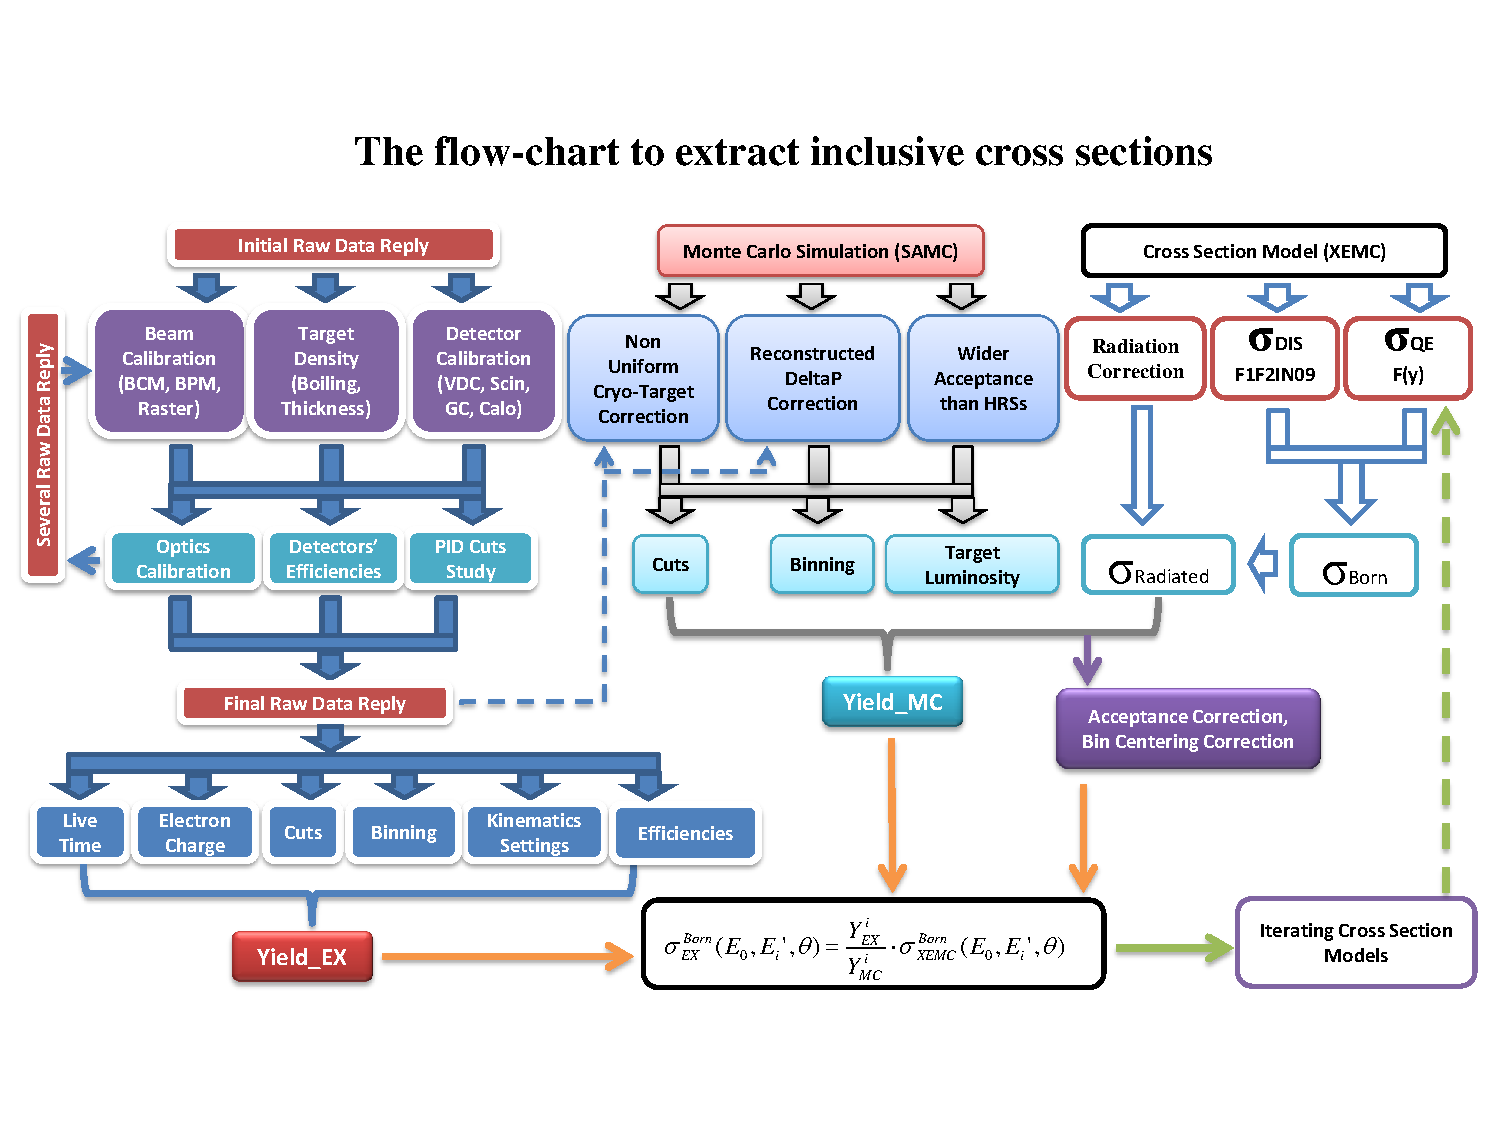
\includegraphics[angle=90, type=pdf, ext=.pdf,read=.pdf,width=1.\textwidth]{./figures/E08014_XS_FlowChart}
  \caption[Flow-chart illustrating cross section extraction]{Flow-chart illustrating cross section extraction}
  \label{xs_flow_chart}
 \end{center}
\end{figure}
The raw cross section in Eq.~\eqref{eqxs_org} requires additional corrections to remove the effects from the spectrometer acceptance. Also, $E_{0}$ and $E'_{i}$ are altered when the electron loses its energy as it passes through the target due to the radiative effects before and after the scattering (see Appendix B.5). The experimental cross section, usually called the radiated cross section, has to be further corrected for radiative effects. The final cross section is the Born cross section, which can be directly compared with theoretical calculations. 

 The basic procedure of extracting cross sections from experimental data is demonstrated in Fig.~\ref{xs_flow_chart}. First of all, the signals from detectors and electronics were stored in the raw data in the form of TDC channels, ADC channels and scaler counts. These signals have to be properly calibrated and converted into applicable quantities. The calibrated HRS optics matrix reconstructs the scattered electron's momentum, scattering angle and reaction point at the target plane. The full set of raw data was replayed with updated parameters in the data base. The calibration of detectors and the HRS optics matrices have been introduced in the previous chapter. 
 
 Secondly, the results of the beam charge monitor (BCM) calibration convert the BCM scaler counts into electron beam charge. The dead-time associated with the DAQ system needs to be evaluated to recover the events lost during the data acquisition. $\eta_{tg}$ is determined by the target thickness after the boiling study. Good electrons are identified by applying cuts on calibrated detector signals, and the efficiencies of the event selection can be individually determined. By binning the data with the kinematic variable, e.g. $E'$, in its proper acceptance range, one can extract the experiment yield in each bin. A description of all the procedures will be given in this chapter.
 
 In addition, the single arm Monte Carlo simulation (SAMC) generates simulation events with the same kinematic settings but with a wider acceptance range to correct the acceptance effect of the HRSs. After weighting the simulation events with the cross sections calculated from model (e.g. XEMC in this experiment), the simulation yields were extracted with the same acceptance cuts and binning method. The Monte Carlo simulation and cross section models will also be discussed in this chapter.

 Finally, the yield ratio method used to extract the cross sections will be introduced, followed by a discussion of errors.

%%%%%%%%%%%%%%%%%%%%%%%%%%%%%%%%%%%%%%%%
% Beam Charge 
%%%%%%%%%%%%%%%%%%%%%%%%%%%%%%%%%%%%%%%%
\section{Beam Charge}
The accumulated electron charge from the beam was monitored by BCMs, where signals were recorded in scalers. The scalers signals, in term of number of counts, have been calibrated~\cite{bcm_patricia} to correctly reflect the accumulated electron charge. When the beam is stable during one run, the total electron charge is simply the product of the beam current and the total run time, and should be directly proportional to the total number of scaler counts. However, events taken during the beam trips must be removed by applying a cut on the electron beam current.

 The average electron beam current in between two consecutive scaler events, called the real-time current, is calculated from the total electron charge collected between these events divided by the time gap. For example, between the $ith$ and the $ith+1$ event, the real-time current measured by the upstream BCM scaler, $\mathrm{U_{1}}$, is given by:
\begin{equation}
  I_{i}^{U_{1}} = \Delta C_{i}^{U_{1}}/\Delta T_{i}, 
\end{equation}
where $\mathrm{\Delta C_{i}^{U_{1}} = C_{i+1}^{U_{1}} - C_{i}^{U_{1}}}$ gives the charge accumulated between two scaler events with the time gap, $\mathrm{\Delta T_{i}=T_{i+1}-T_{i}}$. Similarly, the real-time current measured by the downstream BCM scaler, $\mathrm{D_{1}}$, is also calculated. There are other BCM scaler signals, $\mathrm{U_{3}}$ and $\mathrm{U_{10}}$ ($\mathrm{D_{3}}$ and $\mathrm{D_{10}}$), which basically measure the same charge signal as $\mathrm{U_{1}}$ ($\mathrm{D_{1}}$) but with 3 times and 10 times amplification, respectively. Only $\mathrm{U_{1}}$ and $\mathrm{D_{1}}$ were used since this experiment required very high currents.

 The beam trip cut is applied on the average of these two real-time current values:
\begin{equation}
\frac{1}{2}(I_{i^{*}}^{U_{1}}+I_{i^{*}}^{D_{1}})>I_{beam\_trip\_cut},
\end{equation}
where the cut value can be any value between zero (when beam is tripped) and the value slightly below the maximum current. In this analysis, the beam trip cut was chosen to be 50\% of the normal beam current. The total charge after the beam trip cut is given as:
\begin{equation}
   Q_{e} = \frac{1}{2}\sum_{i^{*}}(\Delta C_{i^{*}}^{U_{1}}+\Delta C_{i^{*}}^{D_{1}}), 
  \label{eq_qe}
\end{equation}
where $i^{*}$ means summing over scaler events with beam current $I_{i^{*}}$ higher than the cut. And the number of electrons in the beam can be calculated as follows:
\begin{equation}
   N_{e} = Q_{e}/e, 
  \label{eq_ne}
\end{equation}
with the electron charge, $\mathrm{e=1.602\times 10^{-19}~C}$.

 After the data replay, scaler events are stored in the scaler trees, \emph{\bf{RIGHT}} for HRS-R and \emph{\bf{LEFT}} for HRS-L, respectively, and they are synchronized with trigger events in the \emph{\bf{T}} tree. There are certain number of trigger events recorded between two consecutive scaler events, and these events are assigned the same value of the real-time beam current evaluated between these two scaler events. Consequently, a beam trip cut removes all trigger events in between two scaler events if the real-time current is lower than the cut.

 During this experiment, BCM scalers on HRS-L did not work properly. Due to the fact that the scalers on both HRSs recorded the same BCM signals, the real-time current for data taken in HRS-L was calculated with scaler events in HRS-R.
%%%%%%%%%%%%%%%%%%%%%%%%%%%%%%%%%%%%%%%%

%%%%%%%%%%%%%%%%%%%%%%%%%%%%%%%%%%%%%%%%
% Dead Time
%%%%%%%%%%%%%%%%%%%%%%%%%%%%%%%%%%%%%%%%
\section{Dead-Time}
  There are two types of dead-time that can cause the loss of events, the electronic dead-time and the computer dead-time. The electronic dead-time comes from the front-end electronics of the DAQ system, which can discard the incoming trigger events while they are busy with processing the current trigger. The computer dead-time is caused by the limitation of computer speed which can lead to the loss of new events when the computer is still writing the current event into the hard disk. Unless the computer is overloaded by processes other than the DAQ system, the computer dead-time is negligible due to the application of high performance computer hardware. 
 
 One evaluates the dead-time as the percentage of the trigger events being discarded to the total trigger events in a certain period of time. The value of the dead-time is directly related to the performance of electronics and computers, but also strongly depends on the total trigger rate. Rather than increasing the hardware performance, a typical method to reduce the dead-time is to limit the total trigger rate below a reasonable value by assigning a pre-scale factor to each trigger. 
 
 The online dead-time during data taking is monitored by using the electron dead-time monitor module (EDTM) which mixes pulse signals with fixed frequency into TDC signals. Within a certain amount of time, the total number of the pulse signals is known and the dead-time value can be given by calculating the percentage of the pulse signals which are not recorded by the DAQ system. By changing the pre-scale factors before the start of the each run, this value was kept under 30\% in this experiment.
 
 The average value of dead-time in each run for the main production triggers was calculated individually during the offline analysis. Although the total number of events recorded by the DAQ system was scaled by the pre-scale factor, their total triggers were counted by scalers, hence the average dead-time for the $ith$ trigger can be given by:
\begin{equation}
  DT_{T_{i}} = 1 - \frac{PS_{T_{i}}\cdot N_{T_{i}}^{DAQ} }{N_{T_{i}}^{Scaler}},
  \label{eq_dt}
\end{equation}
where $PS_{T_{i}}$ is the pre-scale factor of the trigger. $N_{T_{i}}^{Scaler}$ and $N_{T_{i}}^{DAQ}$ are the total number of scaler counts (in $\mathbf{RIGHT}$ tree for $i=1$ or $\mathbf{LEFT}$ tree for $i=3$) and trigger events (in $\mathbf{T}$ tree) for each run, respectively. The beam trip cut was applied when calculating $N_{T_{i}}^{Scaler}$ and $N_{T_{i}}^{DAQ}$.

  A different quantity, live-time ($LT_{T_{i}} = 1 -DT_{T_{i}}$), is more commonly used to correct the total number of good events in each run:
 \begin{equation}
  N^{r}_{T_{i},EX} = PS^{r}_{T_{i}}\cdot \frac{N^{r,recorded}_{T_{i}}}{LT^{r}_{T_{i}}},
  \label{eq_lt}
 \end{equation}
where $r$ denotes the run number; $PS^{r}_{T_{i}}=PS1^{r}$ for the $T_{1}$ trigger on HRS-R and $PS^{r}_{T_{i}}=PS3^{r}$ for the $T_{3}$ trigger on HRS-L; $N^{r}_{T_{i},EX}$ and $N^{r,recorded}_{T_{i}}$ are the number of selected events which create triggers and the number of those events which are recorded by the DAQ system after pre-scaling, respectively. Note that without event selection, e.g. PID cuts, $N^{r,recorded}_{T_{i}}=N^{r,DAQ}_{T_{i}}$.

 In this experiment, since only events from $T_{1}$ ($T_{3}$) were used for data analysis on HRS-R (HRS-L), the subscript, $T_{i}$, is omitted in any future discussion.

%%%%%%%%%%%%%%%%%%%%%%%%%%%%%%%%%%%%%%%%

%%%%%%%%%%%%%%%%%%%%%%%%%%%%%%%%%%%%%%%%
% Target
%%%%%%%%%%%%%%%%%%%%%%%%%%%%%%%%%%%%%%%%
\section{Targets}
 The areal density of scattering centers ( in $\mathrm{cm^{-2}}$) in Eq.~\eqref{eqxs_org} is calculated from the known target thickness:
\begin{equation}
  \eta_{tg} = \frac{\rho\cdot l \cdot N_{a}}{A},
  \label{eq_ntg}
\end{equation}
where $\rho$ is the density of the target material in $\mathrm{g/cm^{3}}$, $l$ is the effective target length in \emph{cm}, $N_{a}$ is the Avogadro's number and A is the nuclear number of the target.
behaviour
\subsection{Cryo-Target Boiling Effect}
\begin{figure}[!ht]
  \begin{center}
    \subfloat[$^{2}H$]{
      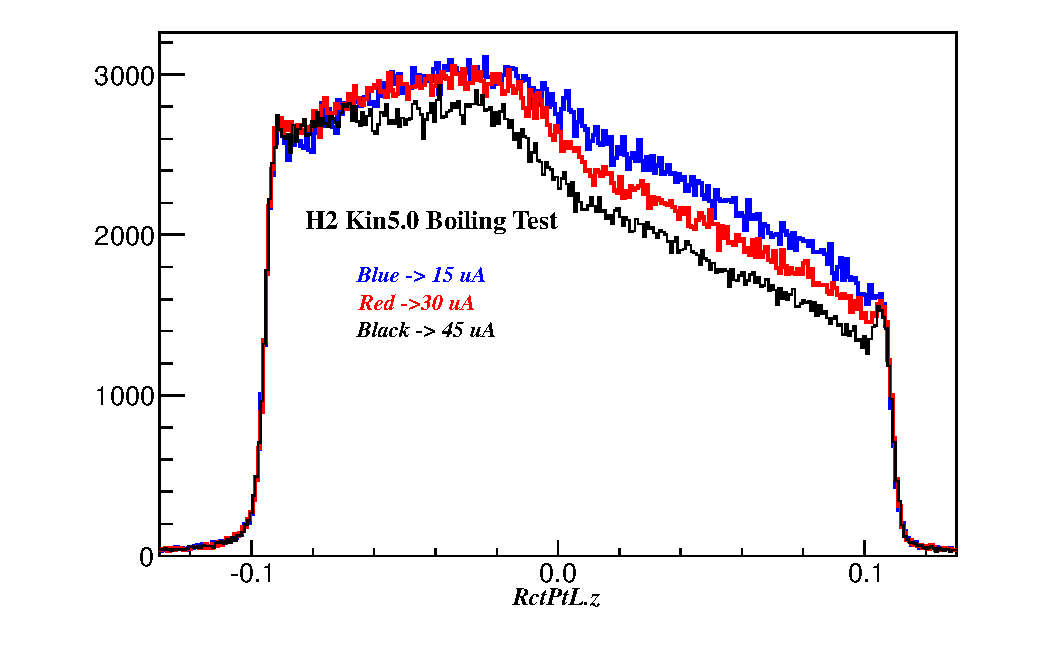
\includegraphics[type=pdf, ext=.pdf,read=.pdf,width=0.62\textwidth]{./figures/target/H2_Boiling_VZ}
    }
    \\
    \subfloat[$^{3}He$]{
      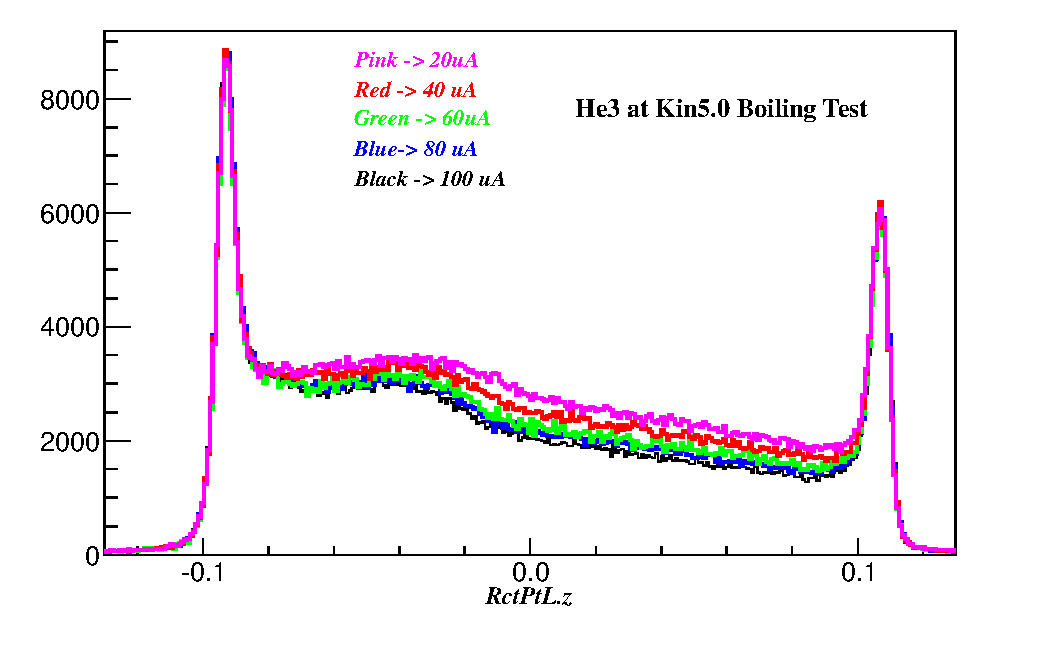
\includegraphics[type=pdf, ext=.pdf,read=.pdf,width=0.62\textwidth]{./figures/target/He3_Boiling_VZ}
    }
    \\
    \subfloat[$^{4}He$]{
      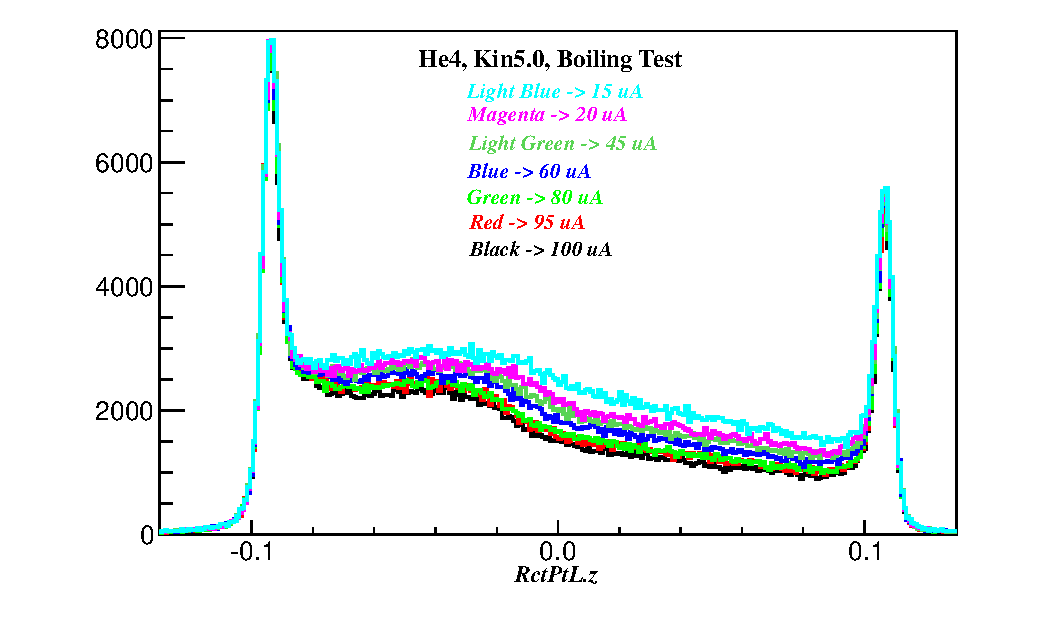
\includegraphics[type=pdf, ext=.pdf,read=.pdf,width=0.62\textwidth]{./figures/target/He4_Boiling_VZ}
    }
    \caption[Cryo-target bumps]{\footnotesize{Cryo-target bumps which appear on the $z_{react}$ distributions because of the non-uniform density of cryo-targets. Due to the boiling effect, the bumps become more significant when the beam current is larger.}}
    \label{bump_current}
  \end{center}
\end{figure}
 When the electron beam passes through the target, the local temperature fluctuates and causes the target density to vary with the beam current. This phenomenon is called the boiling effect. While the density variation of solid targets is usually negligible, liquid and gas targets have significant boiling effects and their densities correlate to the beam current as follow:
\begin{equation}
  \rho = \rho_{0} \cdot (1.0 - B \cdot I /100),
  \label{eq_tgrho}
\end{equation}
where $I$ and $B$ are the values of the beam current and the boiling factor for the target, respectively. $\rho_{0}$ is the nominal target density at $I=0$ and $\rho$ is the actual density with the boiling effect.

 In the E08-014, three cryogenic targets (cryo-targets), $\mathrm{^{2}H}$, $\mathrm{^{3}He}$ and $\mathrm{^{4}He}$, were held in 20 cm long aluminium cells. The cryogenic coolant flowed from the upstream to the downstream of a target cell, and the variation of temperature among different parts of the target leaded to a non-uniform density distribution. When the beam was on, the temperature fluctuation became more significant with higher current. The boiling effect was different along the cryo-target and further increased the non-uniformity of the target densities. Fig.~\ref{bump_current} shows the irregular density distribution and the strong correlation between the density and the beam current. The areal density, $\eta_{tg}$, for these cryo-targets could not be simply calculated from Eq.~\eqref{eq_ntg}.

  A boiling study was performed by dividing each target into several sections along the cell, where the boiling effect was individually evaluated. The relative density distributions were extrapolated from the boiling study results and the absolute target densities were calculated with the survey report of the target system~\cite{target_report}. A detailed discussion is given in Appendix D. 
 
% \subsection{Cryo-Target Cell Contamination}
%%%%%%%%%%%%%%%%%%%%%%%%%%%%%%%%%%%%%%%%

%%%%%%%%%%%%%%%%%%%%%%%%%%%%%%%%%%%%%%%%
% Efficiencies
%%%%%%%%%%%%%%%%%%%%%%%%%%%%%%%%%%%%%%%%
\subsection{Efficiencies}

 Detectors are not in 100\% of performance and the inefficiencies of detectors caused by hardware and software are needed to be evaluated corrected for cross section calculation. 

\subsubsection{Trigger Efficiency}

 There are mainly two aspects that determine the trigger efficiency~\cite{R_Bock}, one of which is the trigger algorithm designed to compromize between highly reducing background rate and keeping most of good events, and the other of which would be the dead time caused by electronics and performance of detectors involved in the trigger system. It is important to avoid double counting detectors' inefficiencies when evaluating trigger efficiencies. The definition of trigger efficiency genrally includes the inefficiency of scintillator counters and the formula is writtern as:

\begin{equation}
 \epsilon_{trigger\_eff} = \frac{PS1(3)\times N_{T1(3)}}{PS1(3) \times N_{T1(3)}+PS2(4)\times N_{T2(4)}},
 \label{trigger_eff}
\end{equation}

where $N_{T1(2,3,4)}$ is number of events triggered by T1(2,3,4) after prescaled by PS1(2,3,4). Tranditionally in Hall-A T1(3) is designed by requesting coincidence trigger signals between S1 and S2m, while T2(4) includes signals from GC in the trigger, which should carry the inefficiency effect of GC. However, during the E08014 experiment, T1(3) was modified to include GC signals in trigger, so the detection inefficiency of GC is canceled from the equation. Fig ~\ref{trig_eff} shows that the trigger efficiencies of our data on both arm were better than 99\%.

%\clearpage
\begin{figure}[h!]
\centerline{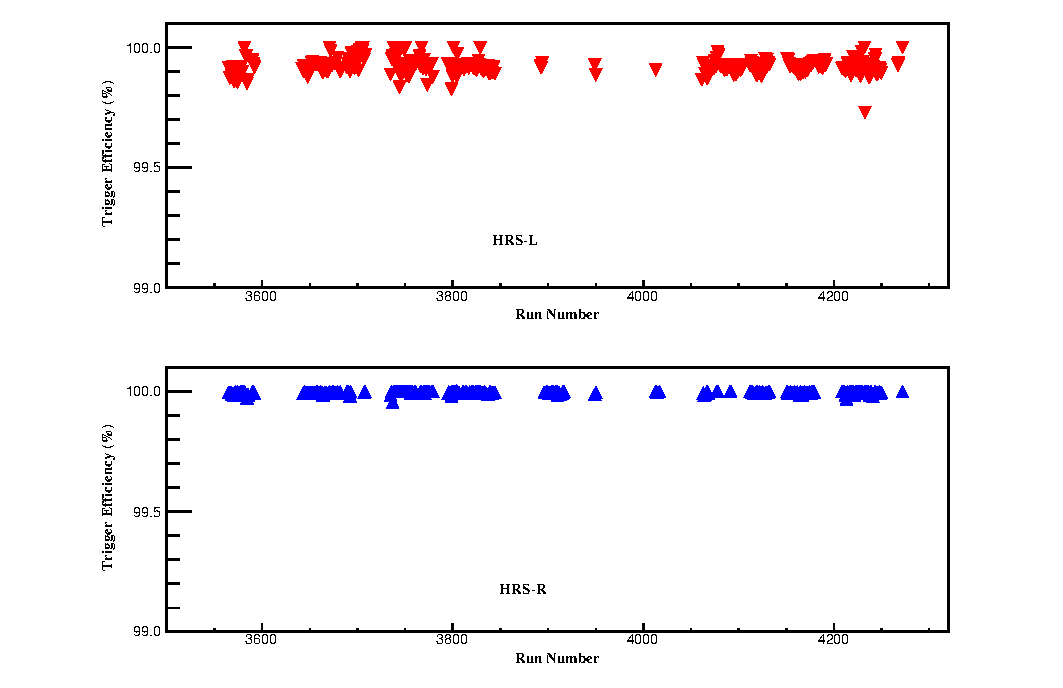
\includegraphics[width=0.7\linewidth]{figures/scin/Trigger_Eff.eps}}
\caption[Trigger Efficiencies]{\footnotesize{Trigger Efficiencies}}
\label{trig_eff}
\end{figure}

\subsubsection{One-Track Efficiency of VDCs}

Inefficiency of VDCs caused by hardware is neglectable and the majore source is from the misreconstruction of particle tracks during the tracking algorithm. Only one-track events are kept for analysis, and the good events threw away by zero-track and multi-tracks cut are corrected by the one-track efficiency defined as:

\begin{equation}
 \epsilon_{one\_track\_eff} = \frac{N_{Track=1}}{N_{0<=Tracks<=4}}
\end{equation}

 It is very important to select correct electron samples when calculating values of one-track efficiency. We need to avoid applying cuts on variables that require trakcing information, such as variables at focal plane and target plane, and cuting on other VDC variables will introduce other sources of inefficiencies. Cluster-reconstructed variables of calorimeters, such as E/P, can not be used when cutting electrons. cosmic ray events should also be removed since they come with big angles. We could not cut on TOF $\beta$ to suppress cosmic ray background due to the TDC multi-peaks issues on some scintillator bars. During the analysis, we used quasi-elastic carbon data which has low cosmic ray backgound due to the high rates,then applied cut on T1(3) trigger, GC ADC sum and Calorimeters ADC sum to select pure electron events, and we also require only one-hit on each scintillator bar for each event to remove events with multi-particles.From Table~\ref{vdc_table}, we obtained the fraction of one-track and multi-track events, which are above 99\% on each arm.

\begin{table}[h!]
\centering
\begin{tabular}{|c||ccccc|}
	\hline
\textbf{Number of tracks}  & 0 & 1 & 2 & 3 & 4     \\
	\hline \hline
HRS-L   & 0.0298\% & 99.1750\% & 0.7430\% & 0.0452\% & 0.0048\%  \\
        \hline
HRS-R   & 0.0482\% & 99.3600\% & 0.5446\% & 0.0388\% & 0.0073\%  \\
	\hline \hline
\end{tabular}
\caption{Fraction of different tracks events from quasi-elastic data,w/o $\beta$ cut}
\label{vdc_table}	
\end{table}



\subsubsection{Detection Efficiencies of PID detectors}
%\subsubsection{Gas Cherenkov}

For Gas Cherenkov detectors and lead-glass Calorimeters, there are two parts of informations needed to be extracted: the fractions of particles detected when they pass throught the detectors and leave signals, or called detection efficiencies; and the percentages of electrons remaining and pions contaiminating when applying PID cuts, also called PID-Cut efficiencies. PID-Cut efficiencies basically tangle with detection efficiencies due to the fact that we deal with detected events. We need to firstly evalute detection efficiencies and PID-Cut efficiencies will be discussed in next section. 

Detection efficiency of GC (Calorimeters) can be defined as:

\begin{equation}
 \epsilon_{detection\_eff}^{cer(calo)} = \frac{N_{detected}^{cer(calo)}}{N_{samples\_from\_calo(cer)}}
\end{equation}

where $N_{cer(calo)}$ is number of particles detected by GC (Calorimeters), and $N_{samples}$ is number of particle samples from Calorimeters (GC). During the analysis, we cut on T1(3) trigger and spectrometer acceptance, and pure electron were selected by applying cuts on main peaks of E/P spectra of Calorimeters when studying GC, or on the peaks of Cherenkov ADC Sum when studying Calorimeters. 

The design of Hall A Gas Cherenkov detectors should give high detection efficiency, since electrons can easily trigger the detectors with very low threshold, while pions and other particles from cosmic ray can not fire the detectors directly, and the inefficiency is caused by particles hitting the edges of gas boxes or PMT tubes. Fig ~\ref{cer_det_eff} shows that on both arm, the detection efficiencies of Gas Cherenkov detectors are close to 100\%.

%\clearpage
\begin{figure}[h!]
\centerline{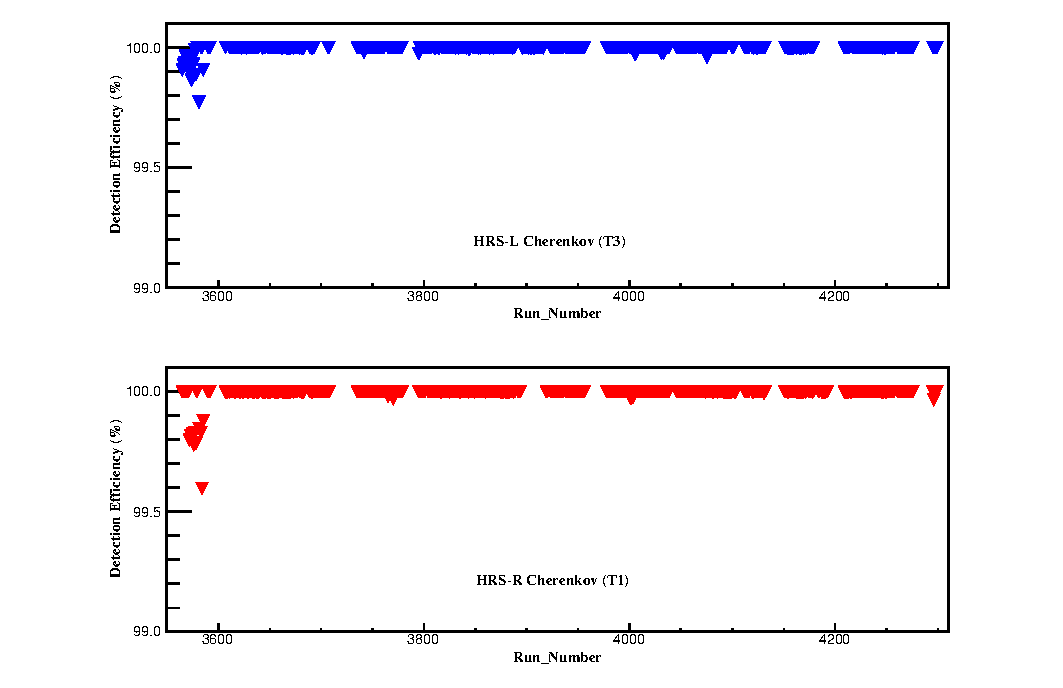
\includegraphics[width=0.7\linewidth]{figures/cer/Cer_Det_Eff.eps}}
\caption[Gas Cherenkov Detection Efficiency]{\footnotesize{Gas Cherenkov Detection Efficiency}}
\label{cer_det_eff}
\end{figure}

%\subsubsection{Calorimeters}
The detection efficiencies of lead glass calorimeters are expected to be lower than Gas Cherenkov detectors. Calorimeters are composed by piles of lead glass blocks, so the inefficiency of detection is mainly from particles going through gaps in between blocks or hitting the edges or PMT tubes before cascade. Cluster reconstruction when calculating deposited energy in lead glass blocks is another source of inefficiencies, especially when the electron rate is low and many low energy cosmic ray particles mix in.From Fig ~\ref{calo_det_eff}, we see that the detection efficiencies of calorimeters on both arm are still high than 99\% for most of runs, but for some runs with low electron rates, mainly for $^{3}He$ target with low beam current (Fig~\ref{calo_det_eff_mom}),the detection efficiencies are slightly lower, due to more cosmic ray contamination. Events from cosmic ray will eventually be removed by applying accpetance cuts and PID cuts, so no correction is necessary for those runs.  

\begin{figure}[h!]
 \centerline{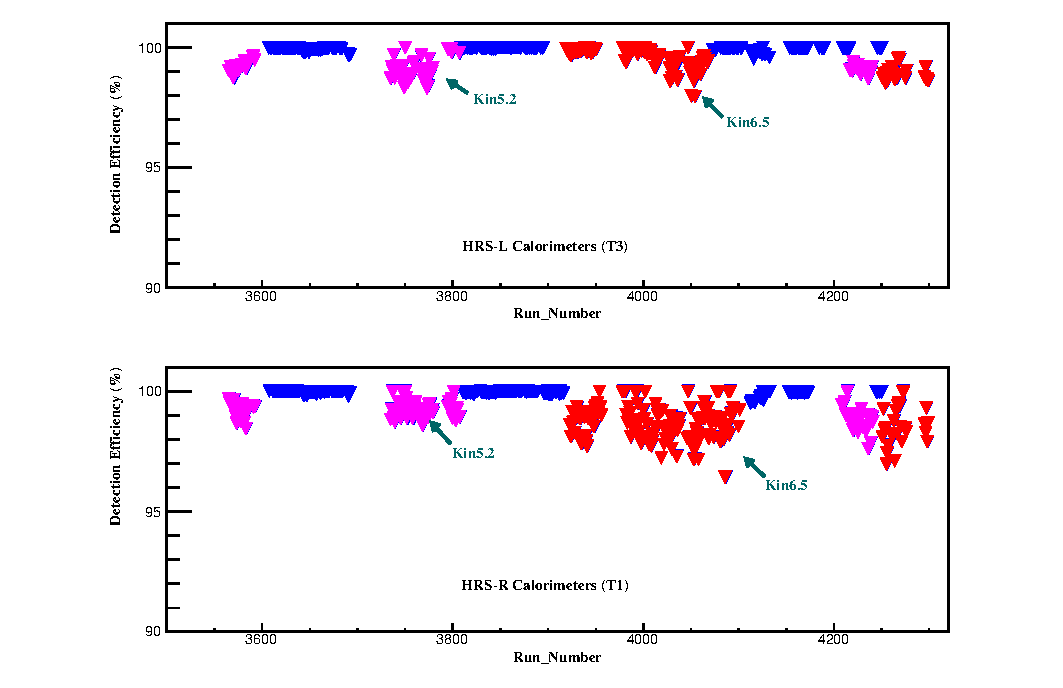
\includegraphics[width=0.7\linewidth]{figures/calo/Calo_Det_Eff1.eps}}
 \captionof{figure}{\footnotesize{Calorimeters: Efficiencies vs Run Number}}
 \label{calo_det_eff}
\end{figure}

\begin{figure}[h!]
 \centerline{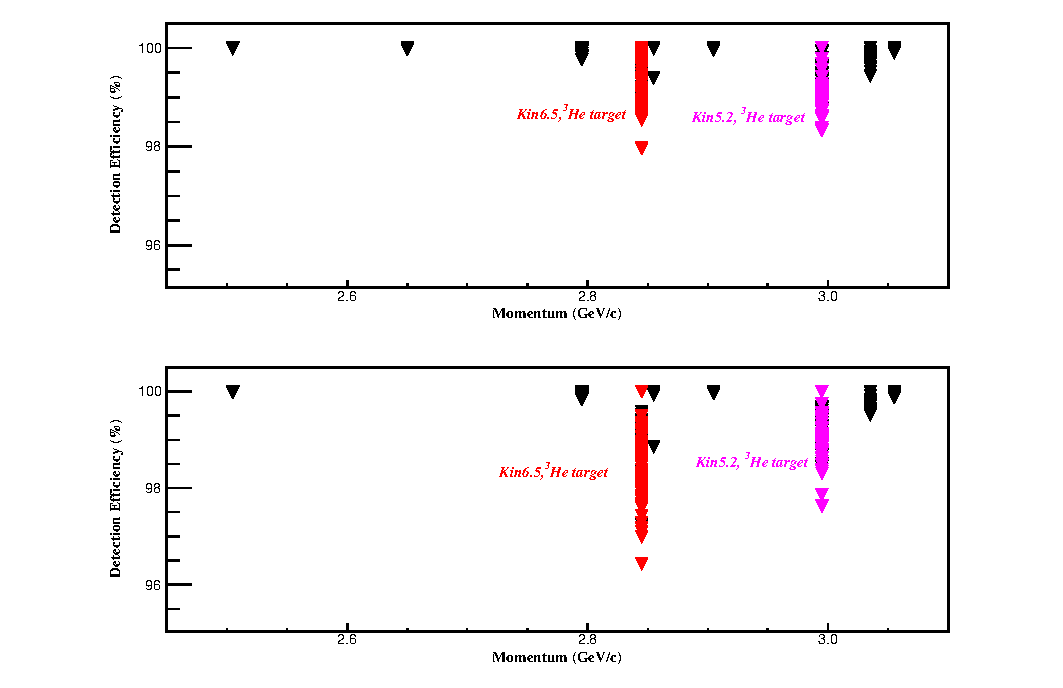
\includegraphics[width=0.7\linewidth]{figures/calo/Calo_Det_Eff_Mom1.eps}}
 \captionof{figure}{\footnotesize{Calorimeters: Efficiency vs Momentum}}
 \label{calo_det_eff_mom}
\end{figure}
%%%%%%%%%%%%%%%%%%%%%%%%%%%%%%%%%%%%%%%%

%%%%%%%%%%%%%%%%%%%%%%%%%%%%%%%%%%%%%%%%
% Cross Section Model & Monte Carlo 
%%%%%%%%%%%%%%%%%%%%%%%%%%%%%%%%%%%%%%%%
\section{Monte Carlo Simulation}
 The Hall-A Single Arm Monte Carlo simulation tool (SAMC) was designed to simulate the transportation of particles from the target plane to the focal plane. SAMC was originally developed in FORTRAN~\cite{A_Duer} and then converted into C++~\cite{hyao_thesis}. The beam position, the spectrometer settings, and the information of the target system can be specified in the code to match the experimental settings. A simulated event has its specified values of the incoming energy, the scattered momentum and the scattering angle, which are defined in the target coordinate system and called the target plane quantities. These quantities are randomly generated with uniform distributions, and with these quantities as inputs, each focal plane quantity is calculated by a set of forward transportation functions which are generated by the SNAKE model~\cite{snack_lerose}. After the focal plane quantities are smeared with the resolution of VDCs, another set of backward transportation functions are used to reconstruct the target plane quantities. During these two processes, events inside and outside the HRS acceptance can be individually identified. Before comparing with the experimental data, the distributions of the target plane quantities are weighted by the radiated cross section values of these simulated events which can be calculated with cross section models embedded in the code. In this analysis, a new cross section model and a special treatment of the no-uniform cryogenic targets have been added in SAMC.

 There were 20 million events generated for each target in each kinematic setting. Fig.~\ref{samc_tg_c12} and Fig.~\ref{samc_tg_he3} compare the distributions of reconstructed target plane quantities between simulated data and experimental data for $\mathrm{^{12}C}$ and $\mathrm{^{3}He}$. The histograms for simulation data were weighted by the cross sections calculated by XEMC (see next section and Appendix B). The distribution of the same quantity from these two data sets agree nicely with each other. The distribution of $z_{react}$ for the cryogenic target was simulated with the relative density distribution function extracted with the method discussed in Appendix D.
\begin{figure}[!ht]
  \begin{center}
    \subfloat[Target plane quantities on HRS-L]{
      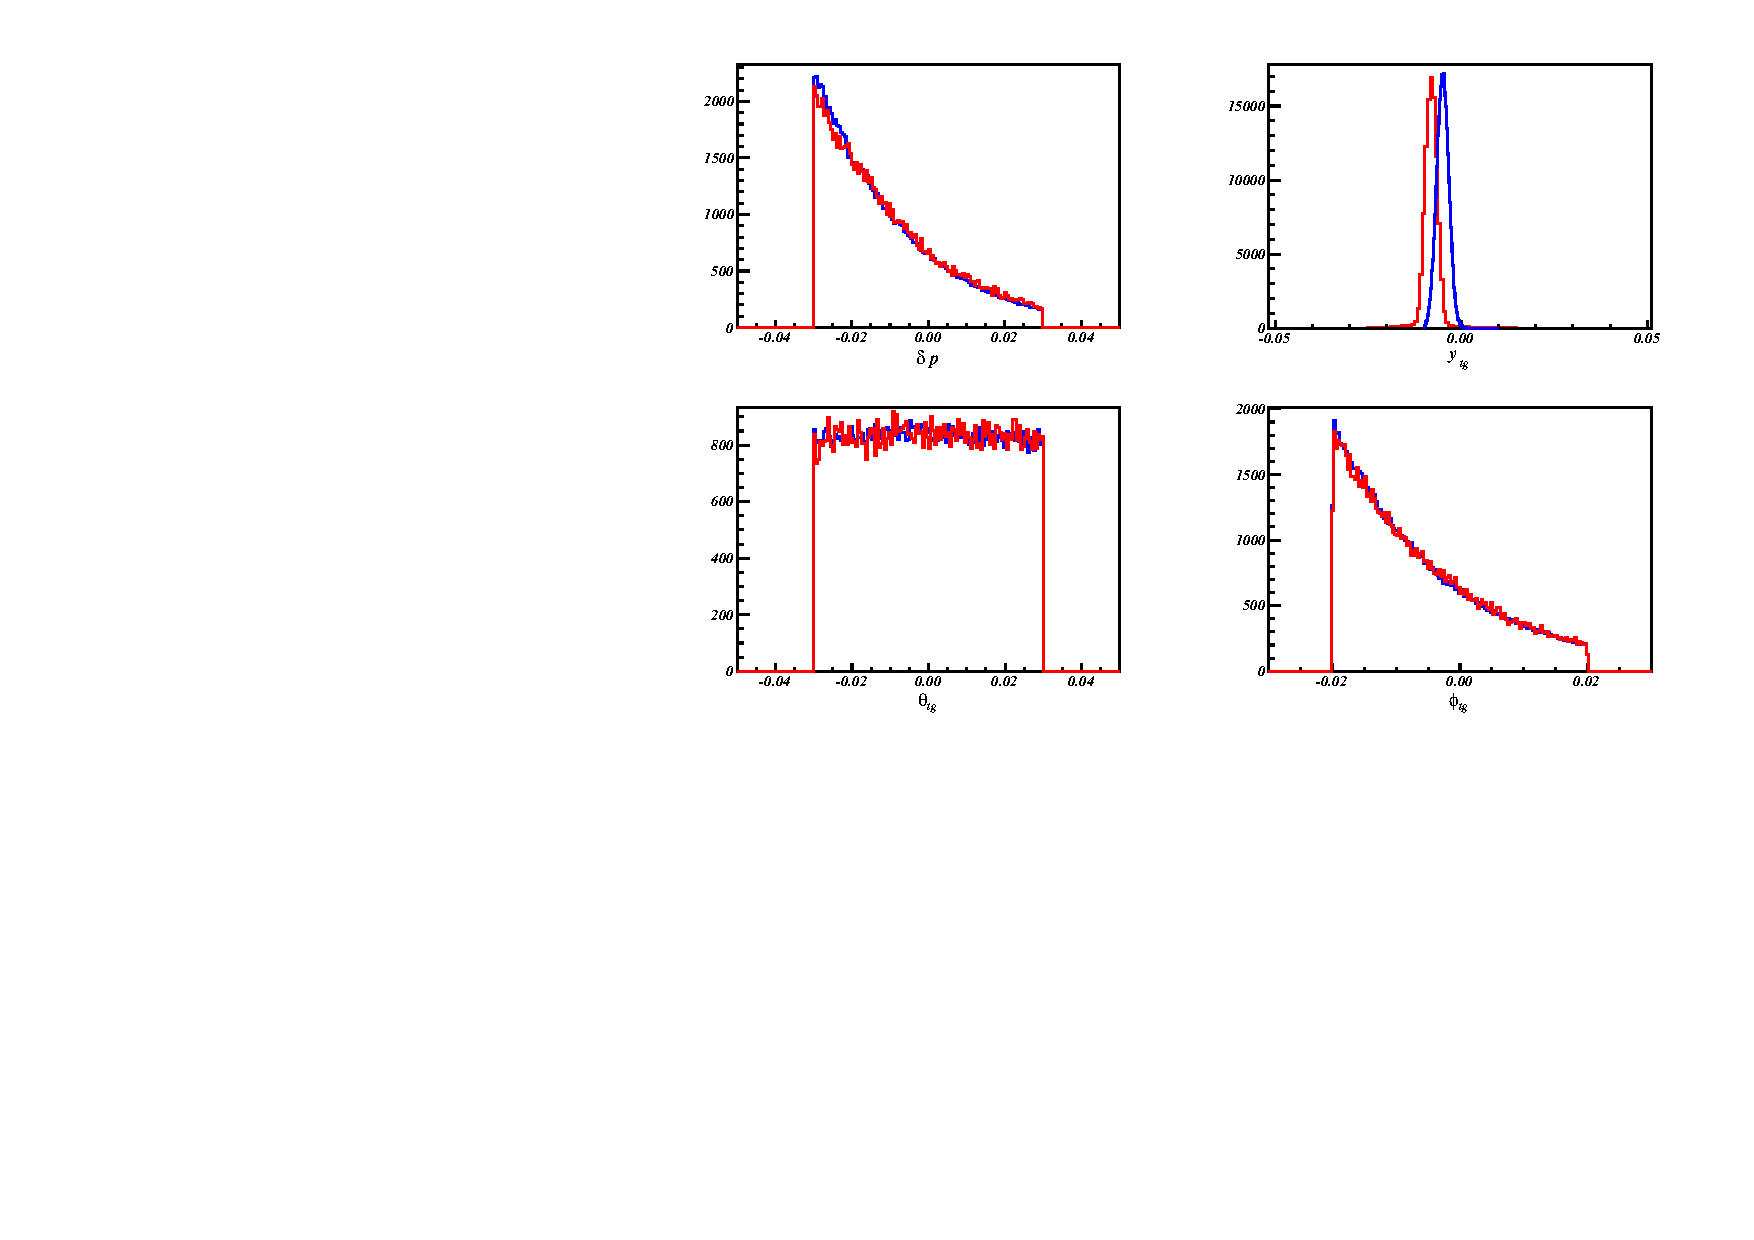
\includegraphics[type=pdf, ext=.pdf,read=.pdf,width=0.92\textwidth]{./figures/samc/C12_L_Kin51_TG}
    }
    \\
    \subfloat[Target plane quantities on HRS-R]{
      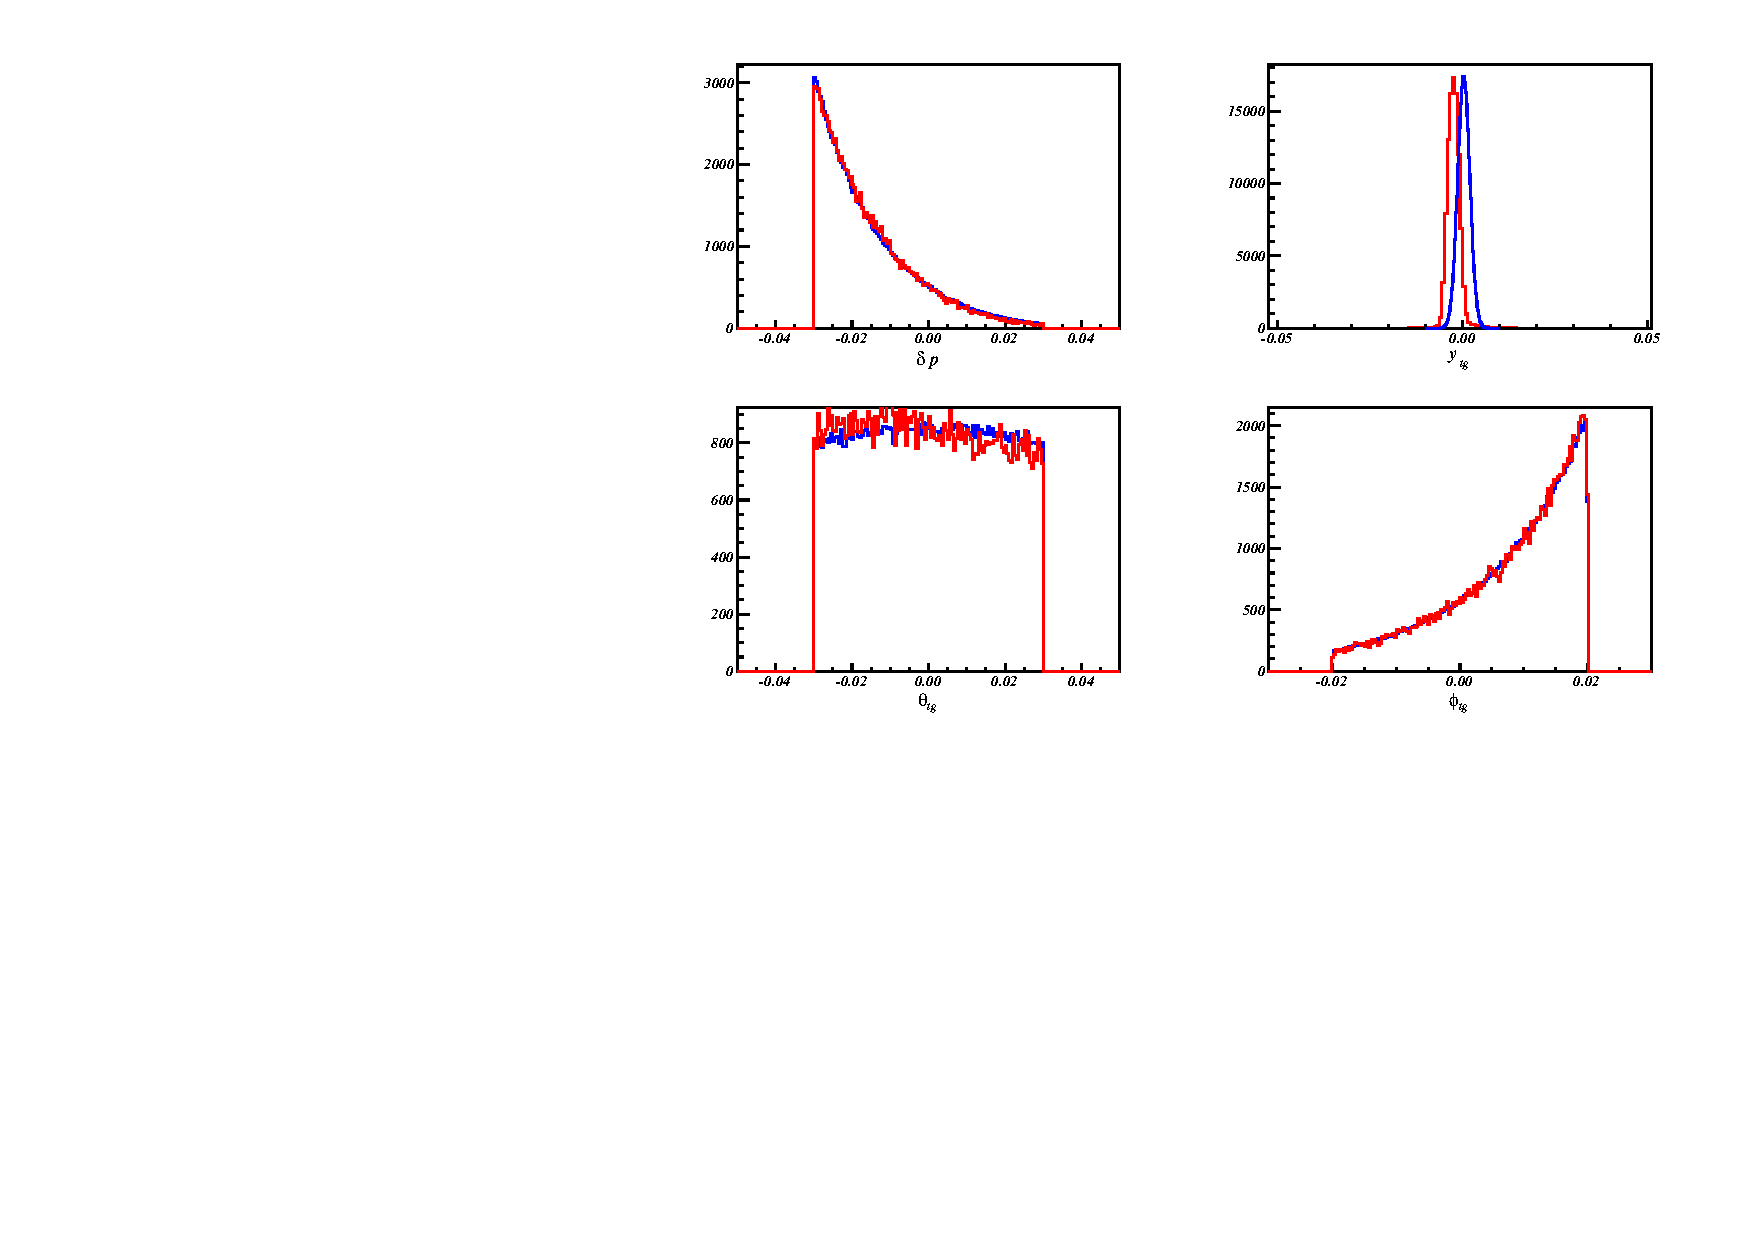
\includegraphics[type=pdf, ext=.pdf,read=.pdf,width=0.92\textwidth]{./figures/samc/C12_R_Kin32_TG}
    }
    \caption[Simulation of $\mathrm{^{12}C}$ target plane quantities]{\footnotesize{Simulation of $\mathrm{^{12}C}$ target plane quantities, where red lines are simulation data from SAMC and blue lines are from the E08-014 data. The offset of $y_{tg}$ between two data is a known issue of SAMC but the offset was too small to affect the acceptance.}}
    \label{samc_tg_c12}
  \end{center}
\end{figure}
\begin{figure}[!ht]
  \begin{center}
    \subfloat[Target plane quantities on HRS-L]{
      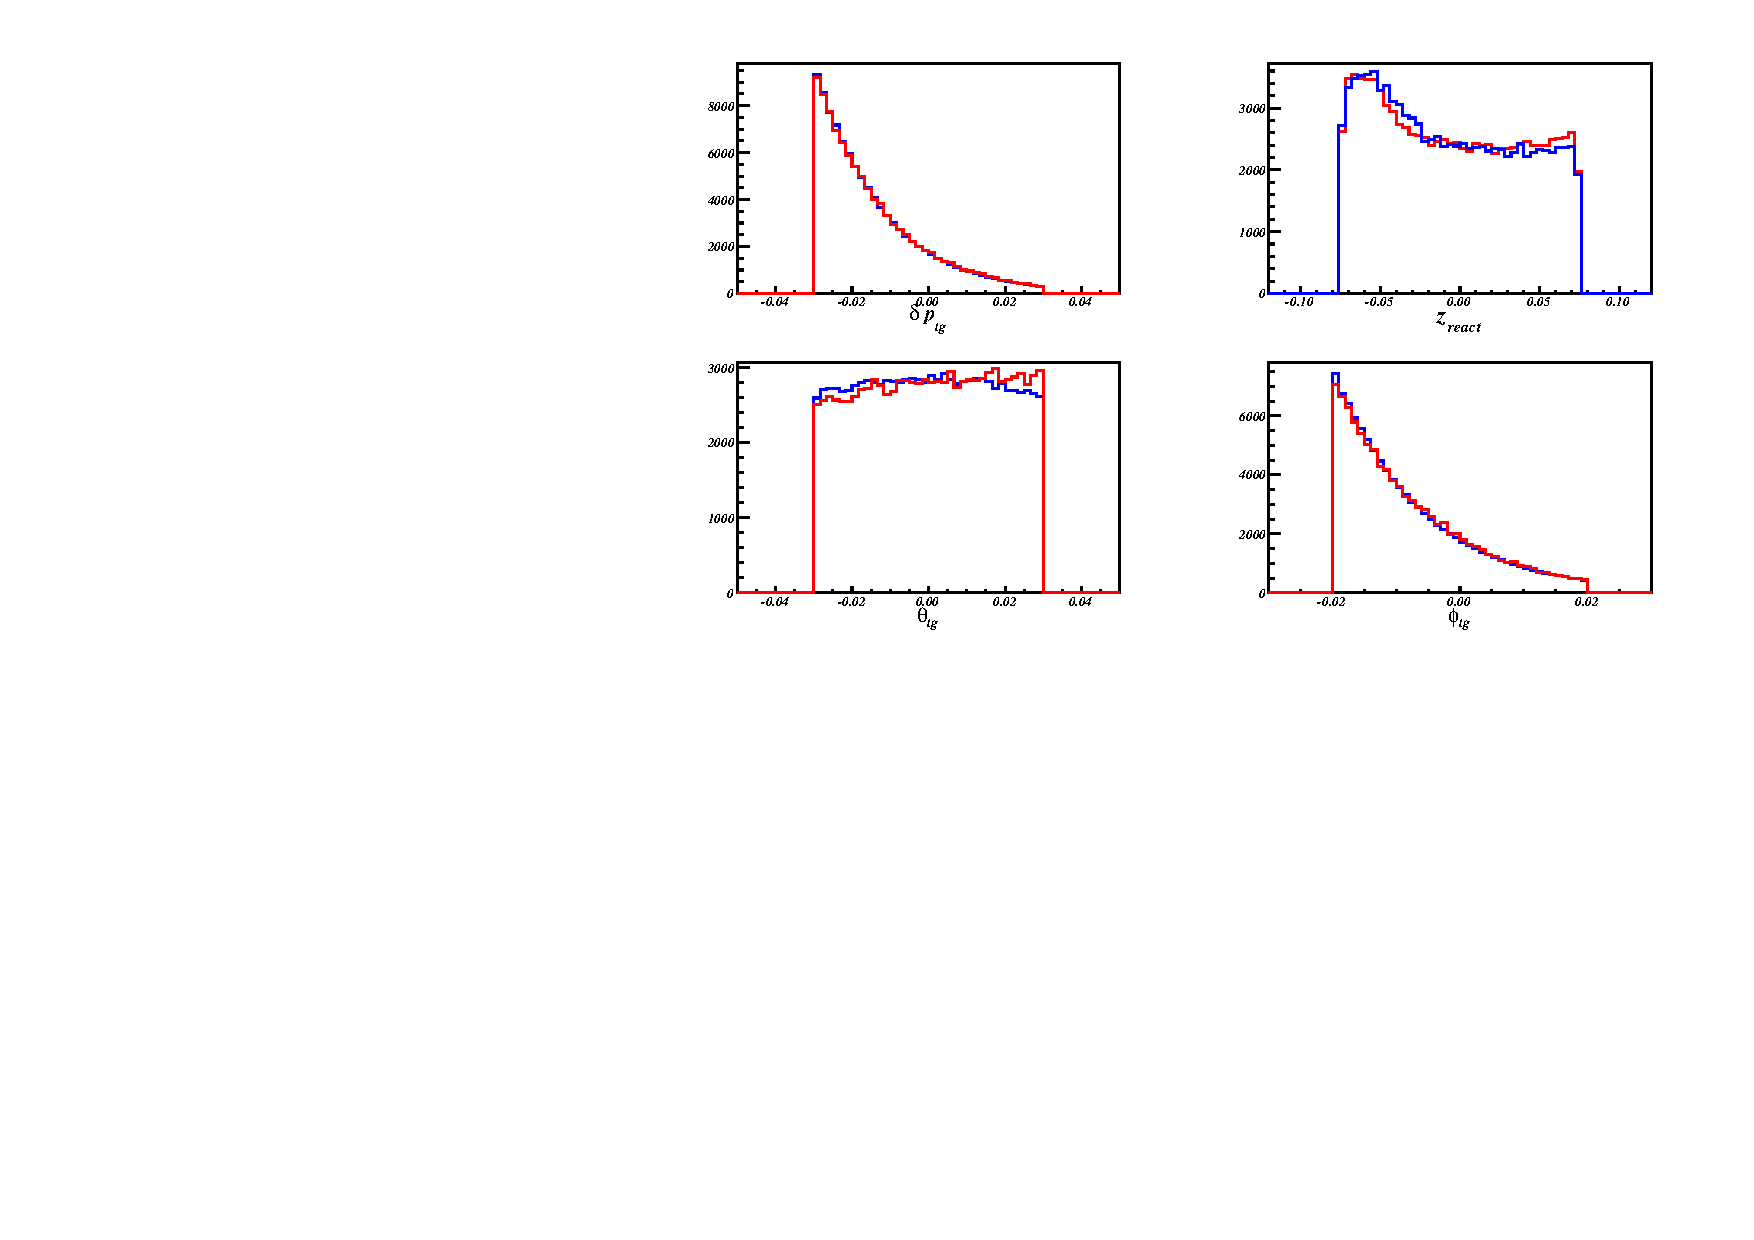
\includegraphics[type=pdf, ext=.pdf,read=.pdf,width=0.92\textwidth]{./figures/samc/He3_L_Kin31_TG}
    }
    \\
    \subfloat[Target plane quantities on HRS-R]{
      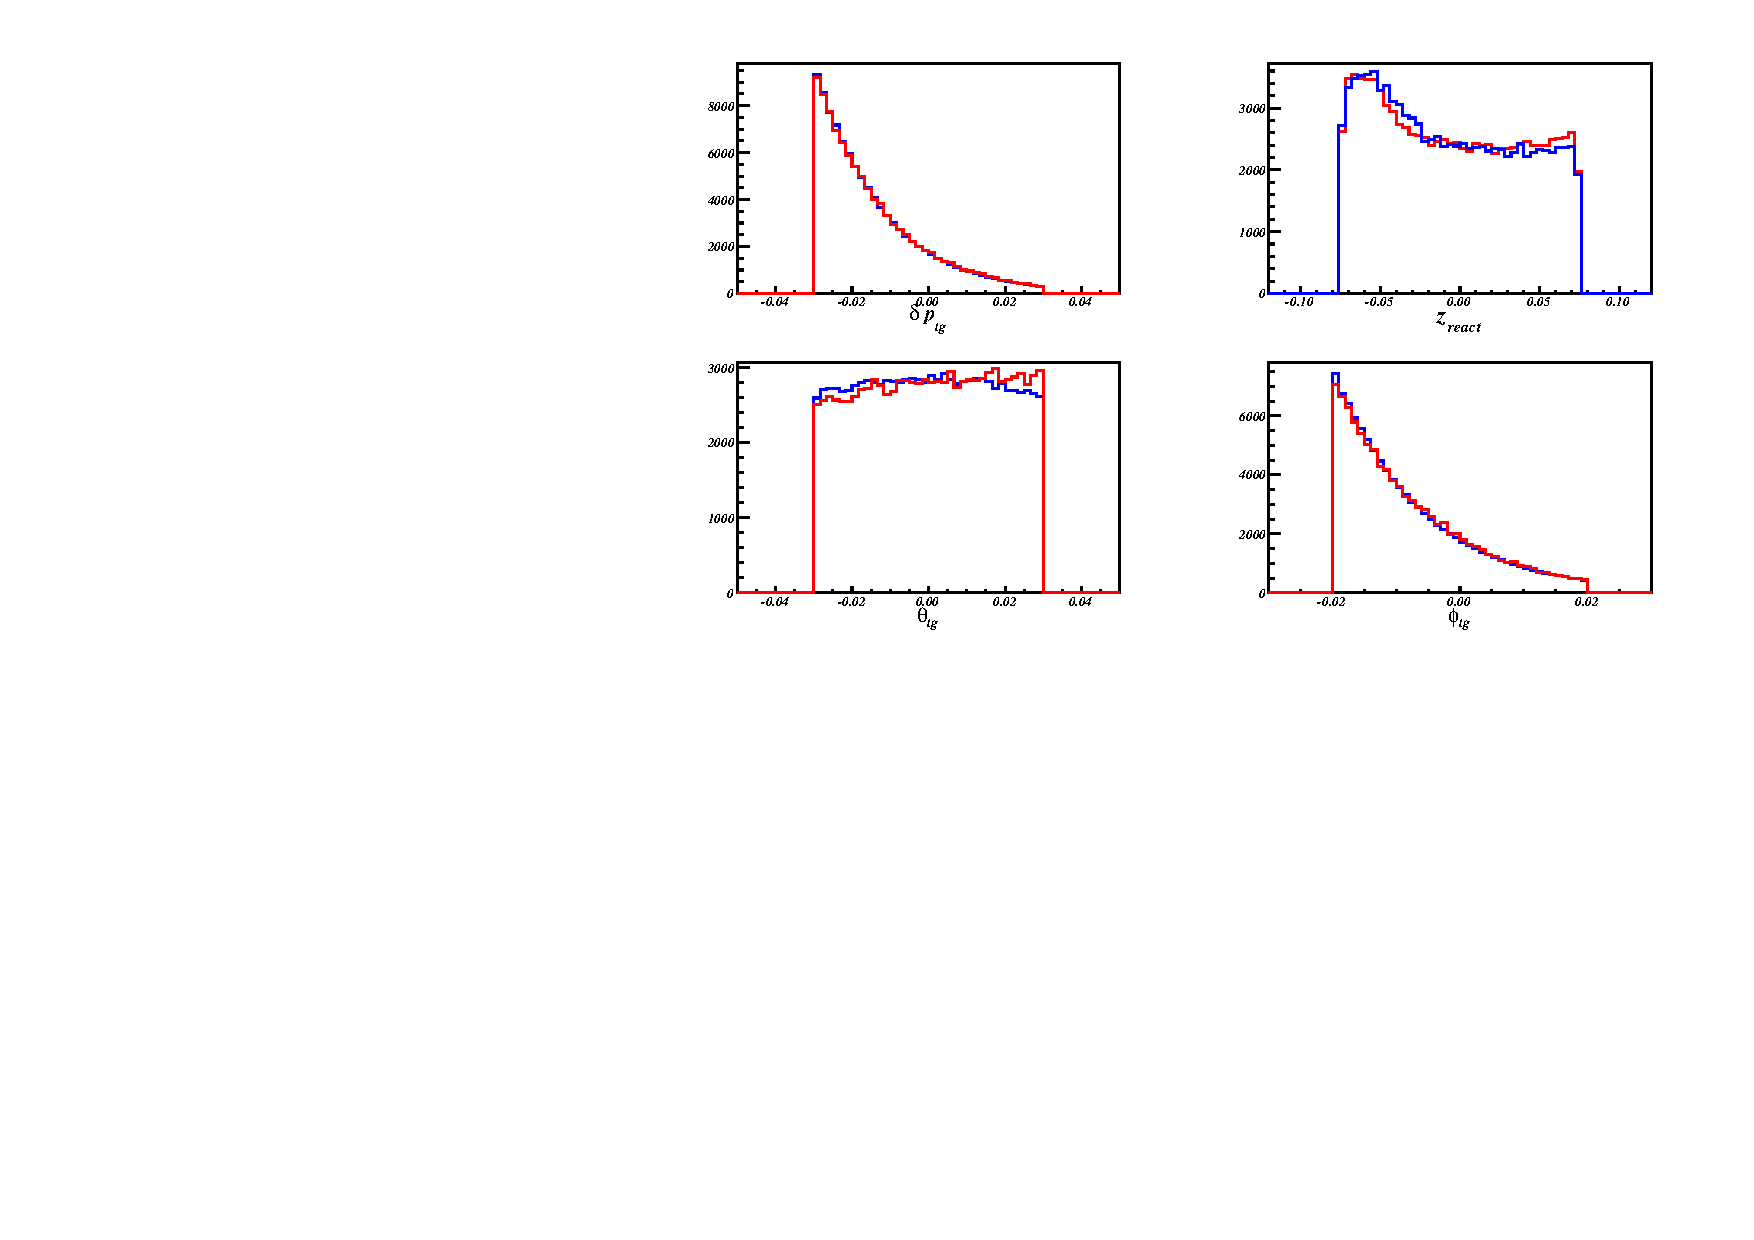
\includegraphics[type=pdf, ext=.pdf,read=.pdf,width=0.92\textwidth]{./figures/samc/He3_L_Kin31_TG}
    }
    \caption[Simulation of $\mathrm{^{3}He}$ target plane quantities]{\footnotesize{Simulation of $^{3}$He target plane quantities, where red lines are simulated data from SAMC and blue lines are the experimental data. Instead of $y_{tg}$, the $z_{react}$ distribution is given to compare the real density distribution which was simulated with the function fitted from data (Appendix D).}}
    \label{samc_tg_he3}
  \end{center}
\end{figure}

\section{Cross Section Model}
 The inclusive electron scattering cross sections model used in this data analysis is XEMC, a C++ package to compute Born cross sections and radiated cross sections. A brief discussion of the cross section models and radiative correction is given in Appendix B. 
\begin{figure}[!ht]
  \begin{center}
    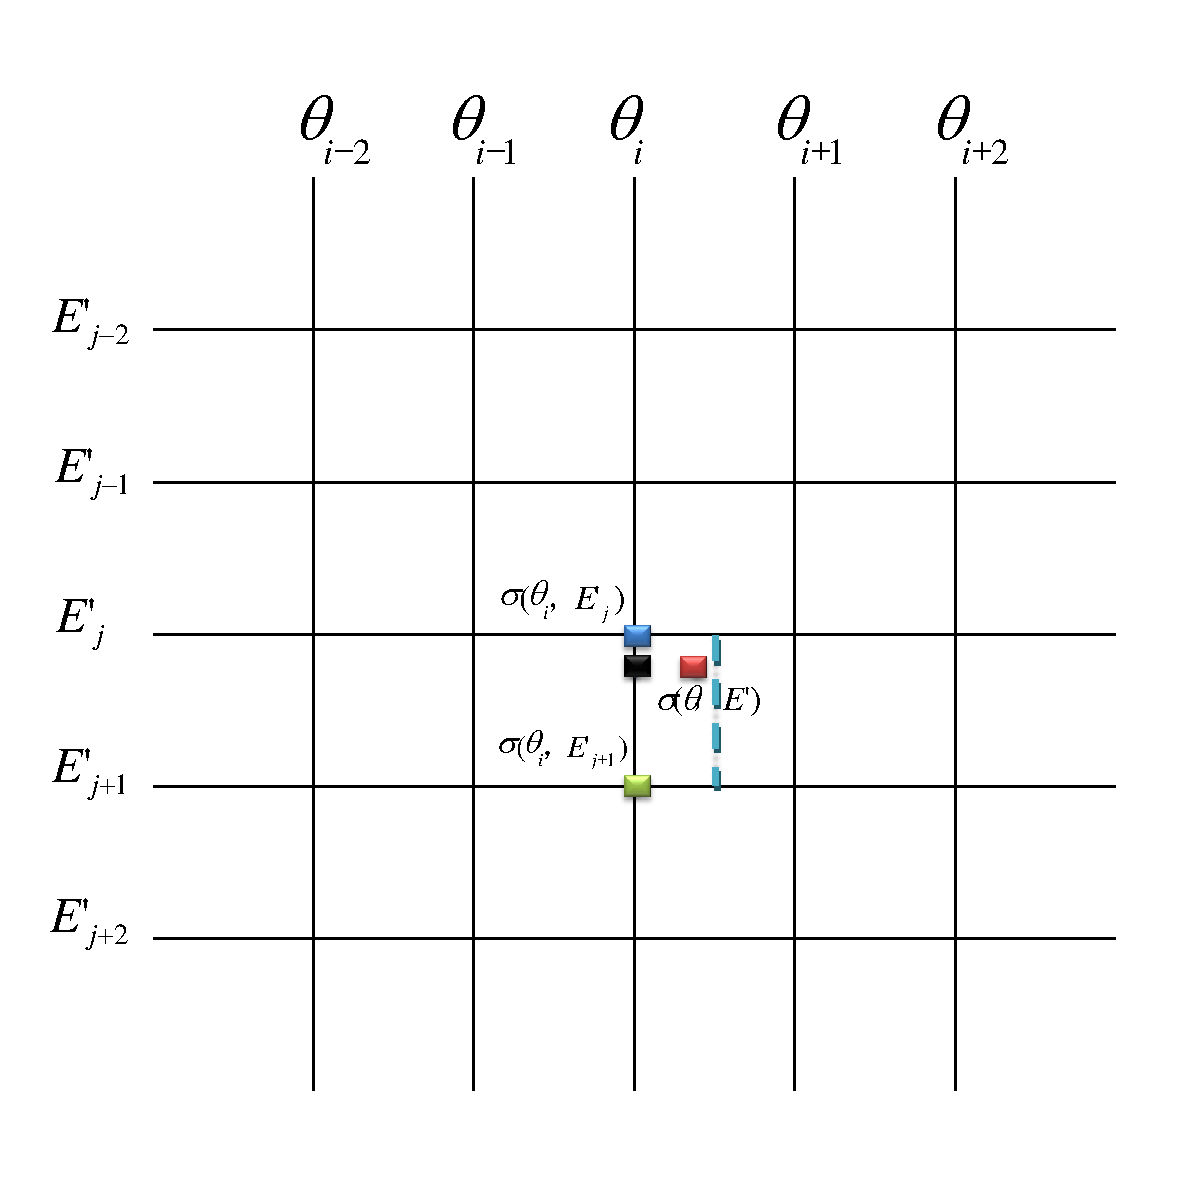
\includegraphics[type=pdf, ext=.pdf,read=.pdf,width=0.60\textwidth]{./figures/xemc/LookUp_Table}
    \caption[A sketch of cross section lookup tables]{\footnotesize{A sketch of cross section lookup tables. $\sigma(\theta,E') \equiv \sigma(\theta_{i},E')$ when $\theta_{i}\leq \theta < (\theta_{i}+\theta_{i+1})/2$, and $\sigma(\theta,E') \equiv \sigma(\theta_{i+1},E')$ when $(\theta_{i}+\theta_{i+1})/2\leq \theta <\theta_{i+1}$, e.g. from the red point to the black point in this plot. For $E'_{j}<E'<E'_{j+1}$, the cross section is calculated with the linear relationship given in Eq.~\eqref{xs_lookup_ep}.}}
    \label{xs_table}
  \end{center}
\end{figure}

 Calculating radiated cross sections with XEMC usually takes very long time. To generate millions of simulated events, cross section look-up tables were generated for each target in each kinematic setting. When generating each table, the range of the scattering angle, $\Delta\theta$, and the scattered energy, $\Delta E'$, were slightly wider than the actual HRS acceptance. $\Delta\theta$ was divided into 200 bins and $\Delta E'$ was also split into bins of 5 MeV. As shown in Fig.~\ref{xs_table}, the kinematic space for each setting was given as a 2-dimensional lattice where the born cross section and the radiated cross section for each grid, ($\theta_{i}$, $E'_{j}$), were simultaneously calculated. Since the bin sizes are very fine, for fixed momentum, the cross sections at different angles are considered to be equal within one $\theta$ bin, while for a fixed angle, the cross sections are assumed to be proportional to the momentum values inside one $E'$ bin. As illustrated in Fig.~\ref{xs_table}, for a given event, ($\theta,E'$), the value of $\theta$ is replaced by the closest angle bin, e.g. $\theta_{i}$, and when two momentum bins are specified, e.g. $E'_{j}<E'<E'_{j+1}$, the cross section value for this event can be calculated with the linear relationship:
\begin{equation}
  \sigma(E',\theta) = \sigma(E'_{j},\theta^{i}) - \frac{E'-E'_{j}}{E'_{j+1}-E'_{j}}\left(\sigma(E'_{j},\theta^{i})-\sigma(E'_{j+1},\theta^{i})\right).
  \label{xs_lookup_ep}
\end{equation}
For the same event, the difference between the cross section obtained from the look-up table and the cross section directly calculated from XEMC is less than 0.1\%. This method can dramatically reduce the computation time when generating simulation events. Tables were re-generated each time when the model was changed or the experimental details were updated, e.g. the target thickness.

%%%%%%%%%%%%%%%%%%%%%%%%%%%%%%%%%%%%%%%%

%%%%%%%%%%%%%%%%%%%%%%%%%%%%%%%%%%%%%%%%
% Yield and Cross Section
%%%%%%%%%%%%%%%%%%%%%%%%%%%%%%%%%%%%%%%%
\section{Event Selection and Corrections}
  The ideal way to extract an experimental cross section is to use the scattered electrons with the same values of $E_{0}$, $E'$ and $\theta$. However, although the beam energy can be easily locked at one value, $E'$ and $\theta$ can vary within the acceptance of the spectrometer, and due to the statistical limitation, the cross sections can only be calculated by allowing the values of $E'$ and $\theta$ to change within finite ranges, e.g. $\Delta E'$ and $\Delta\Omega$ in Eq.~\eqref{eqxs_org}. In practice, the experimental data is divided by binning one or more kinematic variables with known bin sizes, and the cross section is evaluated at the center of each bin. The way to choose the binning method, including the acceptance ranges and the bin sizes, requires additional corrections during the cross section extraction.
   
   For the E08-014, the data was binned in $E'$ only, and the cross sections were calculated in each $E'$ bin with the same scattering angle, $\theta=\theta_{0}$. The determination of the kinematic space, the acceptance correction and the binning correction will be discussed in this section. A list of cuts to select the good electron events is also given.  
  
\subsection{Central Momentum and Angle}
\begin{figure}[!ht]
  \begin{center}
    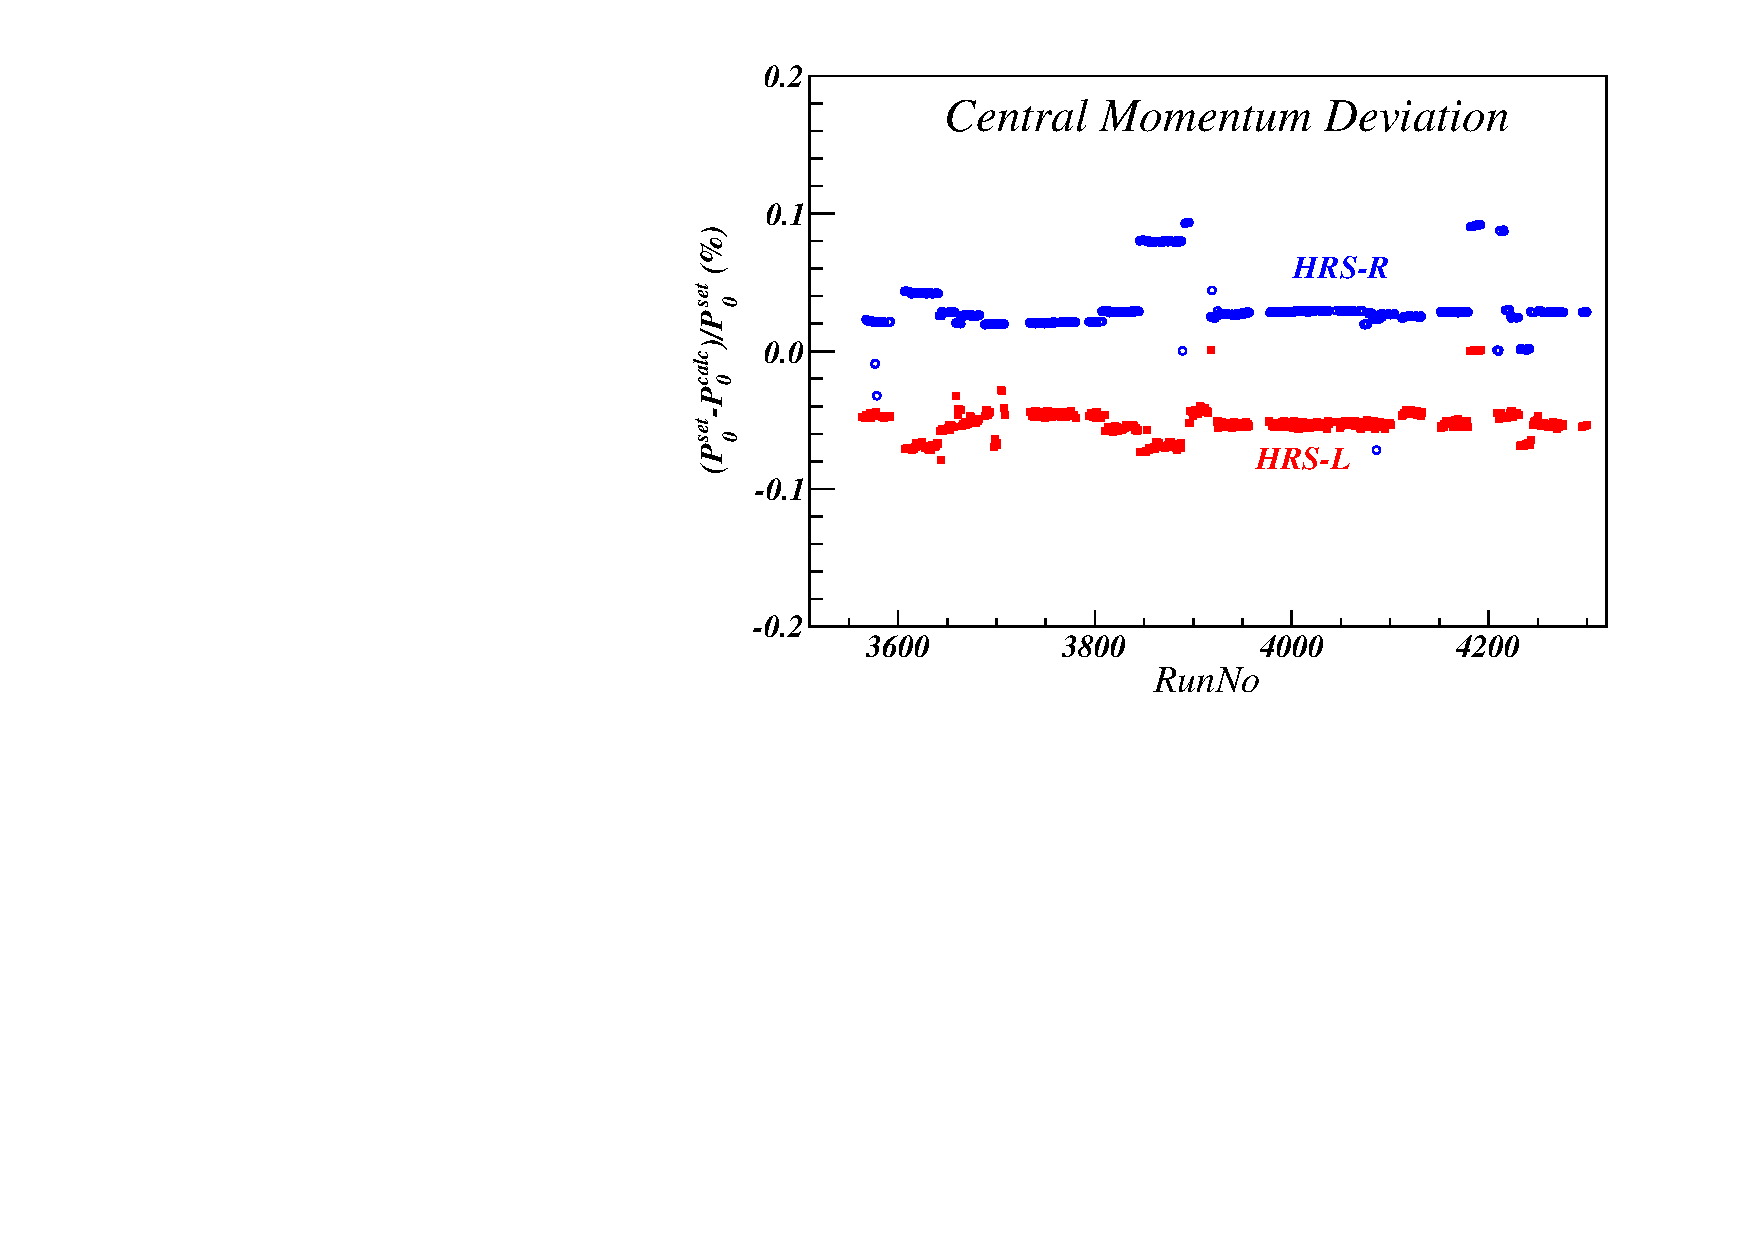
\includegraphics[type=pdf, ext=.pdf,read=.pdf,width=0.60\textwidth]{./figures/xs/point_mom}
    \caption[Central momentum deviation]{\footnotesize{Central momentum deviation, where the blue circles and the red boxes are the deviations of the central momentum on HRS-R and HRS-L, respectively. The x-axis is the run number and the y-axis is the deviation in percentage.}}
    \label{point_mom}
  \end{center}
\end{figure}
The kinematic space is determined by the central scattered momentum, the central scattering angle, and the acceptance of the HRS. The central momentum was given by the field values of the HRS magnets which were locked at the setting values by the HRS NMR system during the experiment. The off-line calculation gives the absolute value of the central momentum with the magnetic field of the dipole~\cite{halla_nim}:
\begin{equation}
 P_{0} = \sum_{i=0}^{4} \gamma_{i} \cdot \left( 10\cdot B^{NMR}_{dipole} \right)^{i},
\end{equation}
where $\mathrm{\gamma_{1,2,3,4}=(0, 270.2, 0, -0.0016)}$ for HRS-L and  $\mathrm{\gamma_{1,2,3,4}=(0, 269.8, 0, -0.0016)}$ for HRS-R. $B^{NMR}_{dipole}$ is the field reading from the NMR monitor. Fig.~\ref{point_mom} shows that the actual central momenta were mostly off by $\pm$3\% while few of them were off by $\pm$10\%. During the cross section extraction, the central momenta were assigned to the calculated values instead of the set values.

The central scattering angle was specified during the experiment by moving the HRS to point at the angle marked on the floor. These floor marks were drawn with respect to the hall center and may not accurately reflect the true values. Moreover, the actual central scattering angle also depends on the offsets between the spectrometer center and the hall center which are different when the spectrometer points at different angles. For some extreme cases, when the spectrometer is moved away from one angle and later moved back to the same value, the actual angles may be different between these two periods.
\begin{table}[!ht]
  \centering
  \begin{tabular}{|c||cccc|}
    \hline
    \textbf{RunNo} &$\theta^{set}_{0}(L)$&$\theta^{true}_{0}(L)$&$\theta^{set}_{0}(R)$&$\theta^{true}_{0}(R)$\\
    \hline \hline
    3565$\sim$3656          & 25.00 & 25.00  & 25.00 & 25.00 \\
    \hline
    3657$\sim$3683          & 21.00 & 21.03  & 21.00 & 21.04 \\
    \hline
     3684$\sim$3708         & 23.00 & 23.00  & 23.00 & 23.01 \\
    \hline
     3735$\sim$3891         & 25.00 & 24.99  & 25.00 & 25.00 \\
    \hline
     3892$\sim$3916         & --    &  --    & 21.00 & 21.03 \\
    \hline
     3917$\sim$4071         & 28.00 & 27.98  & 28.00 & 27.99 \\
    \hline
    4073$\sim$4103          & 21.00 & 21.04  & 28.00 & 27.99 \\
    \hline
    4112$\sim$4179          & 23.00 & 23.00  & 23.00 & 23.04 \\
    \hline
    4181$\sim$4241          & 25.00 & 24.98  & 25.00 & 25.00 \\
    \hline
    4242$\sim$4250          & 21.00 & 21.02  & 21.00 & 21.03 \\
    \hline    
    4251$\sim$4299          & 28.00 & 27.98  & 28.00 & 27.99 \\
    \hline
    \end{tabular}
  \caption{Scattering angle correction}
  \label{scat_angle_table}	
\end{table}

 To obtain the actual central scattering angle each time after the spectrometer was moved, a survey would be performed to correct the errors of the floor marks and to measure the offset between the two centers. Unfortunately, the survey could not been done each time the spectrometers were moved. However, the optics target was surveyed at the beginning of this experiment when both HRSs were set at $\mathrm{25^{\circ}}$, and the positions of $z_{react}$ at different angles can be extracted from the data. Combined with the survey reports from earlier experiments which had similar settings, the actual central scattering angles can be calculated with the difference of $z_{react}$ at $\mathrm{25^{\circ}}$ and at the setting angle ($\Delta z_{react}=z_{react}(\theta_{0})-z_{react}(25^{\circ})$), as follow: 
\begin{eqnarray}
 & &\theta_{tg} = \frac{D_{x}+x_{sieve}-y_{beam}}{L-x_{beam} \cdot sin\theta^{set}_{0}-\Delta z_{react} \cdot cos\theta^{set}_{0}},\\
 & &\phi_{tg}   = \frac{D_{y}+y_{sieve}-x_{beam} \cdot cos\theta^{set}_{0}+\Delta z_{react} \cdot sin\theta^{set}_{0}}{L-x_{beam} \cdot sin\theta^{set}_{0}-\Delta z_{react} \cdot cos\theta^{set}_{0}},\\
 & &\theta^{true}_{0} = acos\left( \frac{cos\theta^{set}_{0}-\phi_{tg}sin\theta^{set}_{0}}{\sqrt{1+\theta_{tg}^{2}+\phi_{tg}^{2}}} \right),
\end{eqnarray}
where $D_{x}$, $D_{y}$, $x_{sieve}$, $y_{sieve}$ and L are given in Table~\ref{optics_offset_table} and Table~\ref{sieve_offset_table}. The beam position ($x_{beam}$, $y_{beam}$) was locked at (-2.668 mm, 3.022 mm) during the experiment. $\theta^{set}_{0}$ is the central scattering reading from the floor marks and $\theta^{true}_{0}$ is the actual central scattering angle after the correction. As shown in Table~\ref{scat_angle_table}, the calculation showed that the maximum offset between $\theta^{true}_{0}$ and $\theta^{set}_{0}$ was not larger than $\mathrm{0.04^{o}}$. The value of $\theta^{true}_{0}$ was calculated for runs taken at each run period when the spectrometer was moved to different positions. The cross sections were calculated with these updated values.

\subsection{Acceptance Correction}
\begin{figure}[!ht]
  \begin{center}
    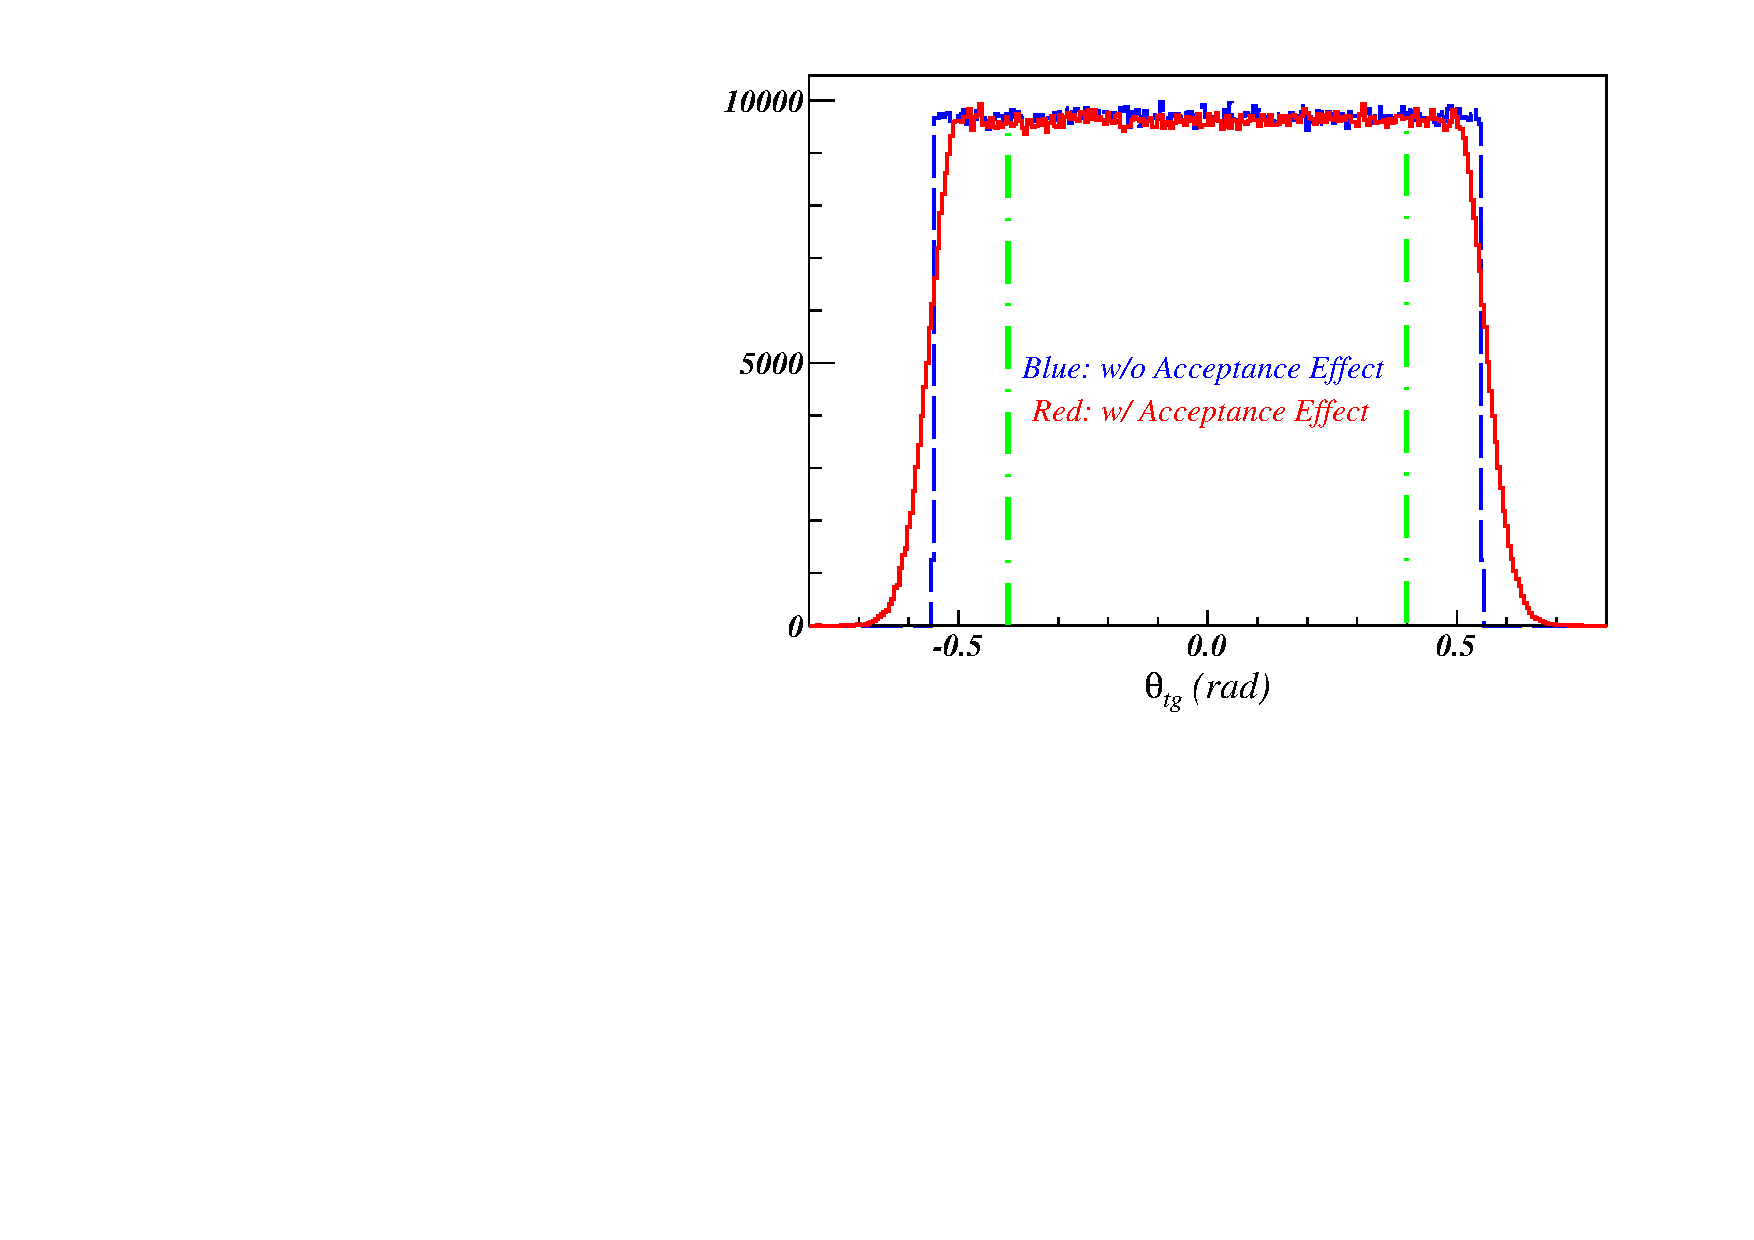
\includegraphics[type=pdf, ext=.pdf,read=.pdf,width=0.60\textwidth]{./figures/xs/accep_demo}
    \caption[A demonstration of the acceptance effect]{\footnotesize{A demonstration of the acceptance effect, where the distribution of $\theta_{tg}$ is generated by assuming no cross section weighting effect. The blue line shows that the acceptance is flat when the HRS acceptance is perfect, while the red line demonstrates the slow fall-off of the acceptance edges. Such an effect is mainly due to the geometry of the HRS magnets and also contributed by the resolutions of the VDC tracking and the optics reconstruction. Green lines show the cuts to select the flat acceptance region.}}
    \label{accp_demo}
  \end{center}
\end{figure}
 The HRS acceptance includes both the range of momentum dispersion ($\Delta\delta p$) and the total solid angle which is the product of the out-of-plane angle ($\theta_{tg}$) and the in-plane-angle ($\phi_{tg}$). For an extended target, the optics reconstructed reaction point along the beam direction ($z_{react}$) is also affected by the HRS acceptance. These four quantities, called the target plane quantities, are essential to reconstruct the reaction at the target. Due to the geometry of the HRS magnets, the event distributions of these quantities are not cut off immediately at the edge of the acceptance and instead, they fall off relatively slowly with a gaussian tail, as can be seen in Fig.~\ref{accp_demo}. In addition, the resolution of VDC tracking and the accuracy of the optics reconstruction can also smear the distributions of these quantities. 
 
 Choosing the right acceptance ranges of the target plane quantities is crucial in order to obtain the correct cross section results. Tight cuts on the target plane quantities were used to select events at the central region of the HRS acceptance. Cutting out the tails on the edges of the focal plane variables also removes multi-scattering events produced inside the spectrometer. The acceptance cuts will be enlarged to increase the statistics of events in one bin, until the cross section results start to deviate from the results calculated with tighter cuts.
 
  However, good events can be incorrectly discarded when one applies the combination cuts of the four target plane quantities to define a valid acceptance region. Such an effect can be corrected by the HRS simulation for each bin:
 \begin{equation}
  A(E_{0},E_{i}, \theta_{0}) = \frac{N^{gen}_{MC}}{\Delta E'_{MC} \Delta\Omega_{MC}}/\frac{N^{i}_{MC}}{\Delta E'_{bin} \Delta\Omega_{EX}},
 \label{acc_corr}  
  \end{equation}
where $\Delta E'_{bin}$ is the bin size of $E'$ and is fixed in both the simulated data and experimental data, and $\Delta\Omega_{EX}$ is the selected angular acceptance range for the experimental data. $N^{i}_{MC}$ is the number of simulated events in the $ith$ bin, with the same acceptance cuts used for the experimental events ($N^{i}_{EX}$) in this bin.  $N^{gen}_{MC}$ is the total number of simulated events without any cuts. $\Delta E'_{MC}$ and $\Delta \Omega_{MC}$ define the full momentum and angular acceptance in the simulation, respectively, and they are slightly larger than the HRS acceptance. Overall,  $\frac{N^{i}_{MC}}{\Delta E'_{bin} \Delta\Omega_{EX}}$ denotes the average number of events in the unit kinematic space which is limited by the HRS geometry, while the other term, $\frac{N^{gen}_{MC}}{\Delta E'_{MC} \Delta\Omega_{MC}}$, gives the average number of events in the unit kinematic space without any spectrometer limitations. Eq.~\eqref{acc_corr} is usually referred to as the acceptance correction. 

\subsection{Binning Correction}
 The cross section results were calculated by binning the data on $E'$. The binning ranges and step sizes are given in the following table:
\begin{table}[!ht]
  \centering
  \begin{tabular}{|c||ccccccccc|}
    \hline
    \textbf{Kin}        & 3.1 & 3.2 & 4.1 & 4.2 &5.0 &5.05 & 5.1 & 5.2 & 6.5 \\
    \hline \hline
    $E'^{Min}$    & 2.76   & 2.90   & 2.71   & 2.88   &2.38   & 2.52   & 2.66   & 2.85   & 2.70   \\
    \hline
    $E'^{Max}$    & 3.05   & 3.21   & 3.00   & 3.19   &2.63   & 2.78   & 2.94   & 3.14   & 2.99   \\
    \hline
    $\Delta E'$      & 0.01   & 0.01   & 0.01   & 0.01   & 0.01  &0.01    & 0.01   & 0.01   & 0.01  \\
    \hline
  \end{tabular}
  \caption{E' binning size and range}
  \label{bin_table}	
\end{table}

  From Eq.~\eqref{eqxs_org}, when binning on $E'$, the cross section in each bin is given as a function of the central scattering angle ($\theta_{0}$) and the momentum value at the center of the bin ($E'_{i}$). However, events in each bin carry different momenta varying from $E'_{i}-\frac{1}{2}\Delta E'$ to $E'_{i}+\frac{1}{2}\Delta E'$ , while their central scattering angles can deviate from $\theta_{0}$ within the solid angle, $\Delta \Omega_{EX}$. A bin-centering correction is applied to remove the effect with the simulation data and the cross section model:
\begin{equation}
 B(E_{0},E_{i}, \theta_{0}) = \frac{\sigma^{rad}_{XEMC}(E_{0},E'_{i},\theta_{0})}{\sum_{j\in i}\sigma^{rad}_{XEMC}(E_{0},E'_{j},\theta_{j})},
  \label{bin_corr}  
\end{equation}
where $\sum_{j\in i}$ means summation over the radiated cross section values, $\sigma(E'_{j},\theta_{j})$), of all Monte Carlo events in the $ith$ bin. $\sigma^{rad}_{XEMC}(E'_{i},\theta_{0})$ and $\sigma^{rad}_{XEMC}(E'_{j},\theta_{j})$ are calculated from the XEMC model.

\subsection{Cuts}
In addition to cutting on the binning variable, there are several other cuts which were applied to select good scattered electron events:
\begin{enumerate}
\item Cutting on production trigger events (see Appendix A);
\item Removing pulser events generated by EDTM modules;
\item Beam trip cut;
\item Selecting events with only one track in VDCs; 
\item Cuts on the focal plane acceptance;
\item Cuts on the target plane acceptance;
\item PID cuts on the GC and the calorimeter.
\end{enumerate}

 When the extraction of cross sections involves data from more than one run, the total number of events after the cuts defined above is given by:
\begin{equation}
  N_{EX}^{i} = \sum_{r} \frac{PS1(3)^{r}\cdot N_{T_{1(3)}}^{r}}{LT_{T_{1(3)}}^{r}},
  \label{eq_nex}
\end{equation}
where $r$ represents the run number and $N_{T_{1(3)}}^{r}$ is the total number of events from $T_{1}$ on HRS-R ($T_{3}$ on HRS-L) and recorded by DAQ after cutting out the beam trip. Note that events from each run are individually corrected by the Live-Time ($LT_{T_{1(3)}}^{r}$) before they are added together.

\section{From Yields to Cross Sections}
The experimental Born cross section can be calculated from Eq.~\eqref{eqxs_org} after applying the acceptance correction (Eq.~\eqref{acc_corr}) and the bin-centering correction (Eq.~\eqref{bin_corr}): 
\begin{equation}
  \sigma^{Born}_{EX} (E'_{i}, \theta_{0}) =  A(E'_{i}, \theta_{0}) \cdot B(E'_{i}, \theta_{0})  \cdot \sigma^{rad}_{EX} (E'_{i}, \theta_{0}) \cdot RC(E'_{i}, \theta_{0}).
  \label{eqxs_org_corr}
\end{equation}
Note that the initial electron energy, $E_{0}$, is fixed at 3.356 GeV during this experiment so it is omitted from the equation. The last term is the radiative correction factor:
\begin{equation}
 RC(E'_{i}, \theta_{0}) = \frac{\sigma^{Born}_{XEMC}(E'_{i},\theta_{0})}{\sigma^{rad}_{XEMC}(E'_{i}, \theta_{0})}.
 \label{eq_radc_fact}
\end{equation}

 Extraction of cross sections from Eq.~\ref{eqxs_org_corr} largely relies on the performance of the simulation and the cross section model, which, however, can not be directly examined from the cross section results. Two useful quantities, the experimental yield and the Monte Carlo (MC) yield, can be extracted to directly compare their differences. The experimental yield is written as:
\begin{equation}
  Y^{i}_{EX} = \frac{N^{i}_{EX}}{N_{e} \cdot \epsilon_{eff}},
  \label{eqyex}
\end{equation}
where $\epsilon_{eff}=\epsilon_{trig}\cdot\epsilon_{vdc}\cdot\epsilon_{e\_cut}^{GC}\cdot\epsilon_{e\_cut}^{calo}$ which are given in Eq.~\eqref{trigger_eff3}, Eq.~\eqref{eq_vdc_eff} and Eq.~\eqref{cut_eff_e}, respectively. The MC yield is given by:
\begin{equation}
  Y^{i}_{MC} = \eta_{tg}\cdot \sum_{j\in i}\sigma^{rad}_{model}(E'_{j},\theta_{j}) \cdot \frac{\Delta\Omega_{MC} \Delta E'_{MC}}{N_{MC}^{gen}}.
  \label{eqymc}
\end{equation}

 The ratio of the experimental yield to the MC yield should be close to one if the performance of the HRS can be well simulated by the MC data and the XEMC model produces cross sections close to the actual values. The experimental Born cross section from Eq.~\ref{eqxs_org_corr} can be rewritten as:
\begin{equation}
  \sigma^{Born}_{EX}(E'_{i}, \theta_{0}) = \frac{ Y^{i}_{EX}}{Y^{i}_{MC}} \cdot \sigma^{Born}_{XEMC}(E'_{i}, \theta_{0}),
  \label{eqxs_ratio}
\end{equation}

The yield ratio method can largely reduce the bias caused by the choice of different cross section models and Monte Carlo simulation tools. While the experimental yield is completely extracted from the data and remains unchanged, one can iterate the cross section model and apply necessary corrections only on the MC yield until the the yield ratio becomes close to one for all $E'$ bins. Furthermore, the acceptance cuts on the HRS can also be studied by varying the cuts and checking the distribution of the yield ratio as a function of the binning variable. Most of other potential issues, such as junk runs, incorrect input parameters and so on, can also be examined in the yield ratio method.

%\subsection{Comparing Yields.}
%  Fig.~\ref{ld2_yield} through Fig.~\ref{ca48_yield} show the distribution of the yields and the yield ratio for all targets used in this experiment. From the ratio plots, the experimental yield and the MC yield agree nicely 

\section{Calculation of Errors}
 One of the most important tasks in the extraction of experimental cross sections is to calculate the systematic errors and statistical errors. Systematic errors are introduced by the experimental instrumentation, the simulation tools and the cross section model, etc. Statistical errors are related to the number of measurements of one quantity during the experiment. It is very important to properly propagate the errors when extracting new quantities from the existing quantities, and any mistakes such as mis-counting or double-counting should be avoided during the cross section extraction. The detailed explanation of the error calculation and propagation is given in the following subsections.

\subsection{Statistical Errors}
 A detailed propagation of statistical errors is discussed here:
\begin{enumerate}

\item \textbf{$N_{e}$:} From Eq.\ref{eq_ne}, since the charge is obtained from the average of two BCM monitor outputs ($U_{1}$ and $D_{1}$),the error is also averaged:
  \begin{equation}
   \delta N_{e}^{r} = \sqrt{\frac{\left(\delta N_{e}^{r,D_{1}}\right)^{2}+\left(\delta N_{e}^{r,U_{1}}\right)^{2}}{2}}
                    = \sqrt{\frac{N_{e}^{r,D_{1}}+N_{e}^{r,U_{1}}}{2}}
                    = \sqrt{\frac{N_{e}^{r}}{2}},
  \end{equation}
where, $r$ means the run number. Hence,
  \begin{equation}
    \delta N_{e} = \sqrt{\sum_{r}\left(\delta N_{e}^{r}\right)^{2}}=\sqrt{\frac{\sum_{r}N_{e}^{r}}{2}}=\sqrt{\frac{N_{e}}{2}}.
  \end{equation}
  
\item \textbf{Live-Time:} Form Eq.\ref{eq_lt}, when  $PS^{r} = 1$:
  \begin{equation}
    \delta LT^{r} = LT^{r} \cdot \sqrt{\frac{1}{N^{r,Scaler}}+\frac{1}{N^{r,DAQ}}},
  \end{equation}
where $PS=PS1$ for HRS-R and $PS=PS3$ for HRS-L. When  $PS^{r} > 1$, the calculation of $\delta LT^{r}$ is given differently~\cite{vince_thesis}:
 \begin{equation}
   \delta LT^{r} = LT^{r} \cdot \sqrt{\frac{1}{N^{r,Scaler}}-\frac{1}{N^{r,DAQ}}}.
 \end{equation}

\item \textbf{$N_{EX}:$} From  Eq.\ref{eq_nex} and $N_{EX}=\sum_{r}N_{EX}^{r}$ for all runs, one gets:
  \begin{equation}
    \delta N_{EX}^{r} = N_{EX}^{r} \cdot \sqrt{\frac{1}{N_{recorded}^{r}} + \left(\frac{\delta LT^{r}}{LT^{r}}\right)^{2} }, \delta N_{EX}=\sqrt{\sum_{r}\left(\delta N_{EX}^{r}\right)^{2}},
  \end{equation}
where $N_{recorded}^{r}$ is defined in Eq.~\eqref{eq_lt}. 

\item \textbf{$Y_{EX}:$} From Eq.\ref{eqyex},
  \begin{equation}
    \delta Y_{EX} =  Y_{EX} \cdot \sqrt{\left(\frac{\delta N_{EX}}{N_{EX}}\right)^{2}+\left(\frac{\delta N_{e}}{N_{e}}\right)^{2}+\left(\frac{\delta\epsilon_{eff}}{\epsilon_{eff}}\right)^{2}},
  \end{equation}
where $\epsilon_{eff}$ is set to one and its statistic error and systematic error are set to zero and 1\%, respectively.

\item \textbf{$Y_{MC}:$} From Eq.\ref{eqymc},
  \begin{equation}
    \delta Y_{MC} =  Y_{MC} \cdot \sqrt{\left(\frac{\delta\sum_{j\in i}}{\sum_{j\in i}}\right)^{2}+\left(\frac{\delta N_{MC}^{gen}}{N_{MC}^{gen}}\right)^{2}},
  \end{equation}
  where $\delta\sum_{j\in i} = \sum_{j\in i}\cdot\frac{1}{\sqrt{N_{MC}^{i}}}$, since it summarizes the cross section of MC events ($N_{MC}^{i}$) in one bin.

\item \textbf{$\sigma_{EX}^{Born}:$} From Eq.\ref{eqxs_ratio},
  \begin{equation}
    \delta \sigma_{EX}^{Born} = \sigma_{EX}^{Born} \cdot \sqrt{\left(\frac{\delta Y_{EX}}{Y_{EX}}\right)^{2}+\left(\frac{\delta Y_{MC}}{Y_{MC}}\right)^{2}}.
  \end{equation}

\end{enumerate}

\subsection{Systematic Errors}
 The entire list of systematic errors has not been determined in this thesis. Few items are given as follows:
\begin{enumerate}
\item \textbf{$\eta_{tg}$:}  Form Eq.~\eqref{eq_ntg} and Eq.~\eqref{eq_tgrho}, there are three quantities that can introduce errors: beam current measurement and calculation ($\delta I$), accuracy of Boiling Factors ($\delta B$), and the accuracy of target thickness measurement ($\delta \rho$). First two terms were temporarily set to zero, hence:
  \begin{equation}
    \delta \eta_{tg} = \frac{\delta\rho}{\rho} \cdot \eta_{tg}.
  \end{equation} 
The value of $\delta \rho$ for each target can be found in Table~\ref{target_table} and in Ref.~\cite{target_report}.
\item \textbf{$\epsilon_{eff}$:}  1\% systematic errors is assigned to each of VDC One-Track efficiency, trigger efficiency, detection and cut efficiencies of Gas \v{C}erenkov and Calorimeters.
%\item \textbf{Optics:}
\item \textbf{$\delta p$ correction (HRS-R only):} The error caused by correcting the un-calibrated $\delta p$ on HRS-R as given in Appendix D has to be evaluated. 0.3\% is assigned in this thesis. The value will be updated in the near future.
\item \textbf{Cross section model and radiative correction:} The error from the cross section models and the radiative correction. An estimation of 3\% is given in this thesis. The value will be updated in the near future.
\end{enumerate}
%%%%%%%%%%%%%%%%%%%%%%%%%%%%%%%%%%%%%%%%

%%%%%%%%%%%%%%%%%%%%%%%%%%%%%%%%%%%%%%%%
% Errors
%%%%%%%%%%%%%%%%%%%%%%%%%%%%%%%%%%%%%%%%
\section{Calculation of Errors}
 In the cross section extraction package, a new type of variable is defined by a C++ class $XGT2\_VAR$, which not only includes the exact value of one quantity but also includes its sysmatic error and statistic error, respectively. When a new quantity is calculated from the operation of other quantities, all sysmatic errors and statistic errors from them will be seperately combined and carried by this new quantity. Comparing with evaluation of total errors after we exact the cross section values, this step-by-step method has its advantage to avoid mistakes such as miss-counting or multi-counting. The detail explaination of errors calculation and propagation is given as follows.

 From Eq.\ref{eqxs_ratio},
  \begin{equation}
  \delta^{stat/sys} \sigma_{EX} = \sigma_{EX} \cdot \sqrt{(\frac{\delta^{stat/sys} Y_{EX}}{Y_{EX}})^{2}+(\frac{\delta^{stat/sys} Y_{MC}}{Y_{MC}})^{2}}
\end{equation}

\subsection{$Y_{EX}:$}
 From Eq.\ref{eqyex},
\begin{equation}
  \delta^{stat/sys} Y_{EX} =  Y_{EX} \cdot \sqrt{(\frac{\delta^{stat/sys} N_{EX}}{N_{EX}})^{2}+(\frac{\delta^{stat/sys} N_{e}}{N_{e}})^{2}+(\frac{\delta^{stat/sys}\epsilon_{\pi/e}}{\epsilon_{\pi/e}})^{2}+(\frac{\delta^{stat/sys}\epsilon_{eff}}{\epsilon_{eff}})^{2}},
\end{equation}
where I always set $\epsilon_{\pi/e} = 1$, and $\epsilon_{eff} = 1$.

\subsubsection{Statistic Errors}
\begin{enumerate}

\item $\delta^{stat} \epsilon_{\pi/e} = 0$

\item $\delta^{stat} \epsilon_{\pi/e} = 0$

\item $\delta^{stat} N_{e} = 0$

\item \textbf{$N_{EX}$}: From  Eq.\ref{eq_lt} and $N_{EX}=\sum_{r}N_{EX}^{r}$ for all runs, we have:
\begin{equation}
  \delta^{stat} N_{EX}^{r} = N_{EX}^{r} \cdot \sqrt{\frac{1}{N_{T_{i}}^{r} PS_{T_{i}}} + (\frac{\delta^{stat} LT_{T_{i}}^{r}}{LT_{T_{i}}^{r}})^{2} }, \delta^{stat} N_{EX}=\sqrt{\sum_{r}(\delta^{stat} N_{EX}^{r})^{2}}
\end{equation}

\end{enumerate}

\subsubsection{Systematic Errors}
\begin{enumerate}

\item $\delta^{sys} \epsilon_{\pi/e} = 0.01$

\item $\delta^{sys} \epsilon_{\pi/e} = 0.01$

\item From Eq.\ref{eq_ne}, since the charge is obtained from the average of four BCM monitor outputs ($u_{1},u_{3},d_{1}$ and $d_{3}$),the error is also averaged:
\begin{eqnarray*}
  \delta N_{e}^{r} &=& \sqrt{\frac{(\delta N_{e}^{r,d_{1}})^{2}+(\delta N_{e}^{r,d_{3}})^{2}+(\delta N_{e}^{r,u_{1}})^{2}+(\delta N_{e}^{r,u_{3}})^{2}}{4}}\\
                  &=& \sqrt{\frac{N_{e}^{r,d_{1}}+N_{e}^{r,d_{3}}+N_{e}^{r,u_{1}}+N_{e}^{r,u_{3}}}{4}}\\
                  &=& \frac{\sqrt{N_{e}^{r}}}{2} \\
\end{eqnarray*}
Hence,
\begin{equation}
  \delta N_{e} = \sqrt{\sum_{r}(\delta N_{e}^{r})^{2}}=\frac{1}{2}\sqrt{\sum_{r}N_{e}^{r}}=\frac{1}{2}\sqrt{N_{e}},
  \label{eq:beam_charge}
\end{equation}
where, $r$ means the run number.

\item $\delta^{sys} N_{EX} = N_{EX} \cdot \sqrt{ \sum_{r} (\delta^{sys} LT^{r}/LT^{r})^{2}}$. Form Eq.\ref{eq_lt},
\begin{equation}
  \delta^{sys} LT^{r}_{T_{i}} = LT^{r}_{T_{i}} \cdot \sqrt{\frac{1}{N_{T_{i}}^{Scaler}}-\frac{1}{N_{T_{i}}^{DAQ} PS_{T_{i}}}},
\end{equation}
where there is one thing that confuses me, which is that whether I should multiply $PS_{T_{i}}$ in the first term or not. It won't give us problem so far since most of runs have PS equal to one.

\end{enumerate}

\subsection{$Y_{MC}:$} 

From Eq.\ref{eqymc},
\begin{equation}
  \delta^{stat/sys} Y_{MC} =  Y_{MC} \cdot \sqrt{(\frac{\delta^{stat/sys} N_{tg}}{N_{tg}})^{2}+(\frac{\delta^{stat/sys}\sum_{j\in i}}{\sum_{j\in i}})^{2}+(\frac{\delta^{stat/sys} N_{MC}^{gen}}{N_{MC}^{gen}})^{2}},
\end{equation}

\subsubsection{Statistical Errors}
 Statistical errors from all three terms are set to zero.

\subsubsection{Systematic Errors}

\begin{enumerate}


\item Form $N_{tg} = \frac{\rho\cdot l \cdot N_{a}}{A}$, and $\rho_{cor} = \rho \cdot (1.0 - B \cdot I /100)$, there are three terms that can introduce errors: beam current measurement and calculation ($\delta I$), acuracy of Boiling Factors ($\delta B$), and the acuracy of target thickness measurement ($\delta \rho$). Last term is known but I temperately set the first two terms to zero. Hence:
 \begin{equation}
    \delta N^{sys}_{tg} = \frac{\delta\rho}{\rho} \cdot N_{tg}
 \end{equation} 

\item $\delta^{sys}\sum_{j\in i} = (\sum_{j\in i})\cdot\frac{1}{\sqrt{N_{MC}^{i}}}$, since it is sumarizing the cross section values of MC events ($N_{MC}^{i}$) in one bin.

\item $\delta^{sys} N_{MC}^{gen} = \sqrt{N_{MC}^{gen}}$. I generated $2\cdot 10^{7}$ events for cryogenic targets and $5\cdot 10^{6}$ for foil targets.

\end{enumerate}

\subsection{Systematic Table}
 
 \begin{table}[htbp]
 \centering
    \begin{tabular}{|l|c|c|c|c|}
    \hline
     Source               & Scale & Relative & $\delta\sigma/\sigma$& Comment   \\[6pt]
  \hline
    \hline
    Trigger Efficiency    &      &     $<$1.0\%  &                      &          \\[7pt] \hline
    Tracking Efficiency   &      &     $<$1.0\%  &                      &          \\[7pt] \hline
    GC Efficiency         &      &     $<$1.0\%  &                      &          \\[7pt] \hline
    Calo Efficiency       &      &     $<$1.0\%  &                      &          \\[7pt] \hline
 %   PID Cut Efficiency    &      &          &                      &          \\[5pt] \hline
     Dead Time             &      &     $<$0.4\%     &                      &      \\[7pt] \hline
    Pion Contamination (PID)    &      &          &                      &          \\[7pt] 
    \hline
    \hline
    Acceptance Correction       &      &          &                      &          \\[7pt] \hline
    Bin-Centering Correction    &      & $<$1.0\% &                      &          \\[7pt] \hline
    Radiative Correction        &      &          &                      &          \\[7pt] \hline
    Coulomb Correction          &      &          &                      &          \\[7pt]
    \hline
    \hline
    HRS Momentum         &      &   0.02\%      &                      &          \\[7pt] \hline
    HRS Angle            &      &   $<$0.5mrad  &                      &          \\[7pt] \hline
    Beam Energy          &      &   0.05\%      &                      &          \\[7pt] \hline
    Beam Charge          &      &   $<$1.0\%    &                      &          \\[7pt] 
   \hline
    \hline
    Target Density       &      &          &                      &          \\[7pt] \hline
    Target Boiling       &      &          &                      &          \\[7pt] \hline
    Dummy Subtraction    &      &          &                      &          \\[7pt] 
    \hline
    \hline
    Total               &       &          &                      &          \\[7pt]
    \hline
    \end{tabular}
      \caption{E08-014 systematic error table}
  \label{sys_table}
  \end{table}
  
  \clearpage
\subsection{Systematic Errors in Cross Section Ratio}

The spread-out formula of the experimental differential cross section is given as:
\begin{equation}
  \sigma_{EX} = \frac{Y_{EX}}{Y_{MC}}\sigma_{XEMC}=\frac{N_{EX}}{N_{e}\cdot \epsilon_{eff}} \frac{N_{MC}}{\eta_{tg}\cdot \sum_{j\in i}\sigma^{rad}_{model}(E'_{j},\theta_{j}) \cdot \Delta\Omega_{MC} \Delta E'_{MC}}\cdot\sigma_{XEMC}.
\end{equation}
To decompose each term, we have:
\begin{equation}
 \sigma_{EX} = N_{EX}\cdot N_{e}^{-1}\cdot \epsilon_{eff}^{-1}\cdot (N_{MC})^{-1}\cdot\eta_{tg}^{-1}\cdot (\sum_{j\in i}\sigma^{rad}_{model}(E'_{j},\theta_{j}))^{-1}\cdot\sigma_{XEMC}\cdot (\Delta\Omega_{MC} \Delta E'_{MC})^{-1}.
\end{equation}

Now let's sort out the sources of the systematic error for the cross section:
\begin{equation}
  \delta \sigma_{EX} = \delta N_{EX} \oplus\delta N_{e}^{-1} \oplus\delta \epsilon_{eff}^{-1}\oplus\delta (N_{MC})^{-1}\oplus\delta\eta_{tg}^{-1}\oplus\delta (\sum_{j\in i}\sigma^{rad}_{model}(E'_{j},\theta_{j}))^{-1},
\end{equation}
where $\oplus$ stands for a quadric sum between two uncorrelated errors, e.g. $\delta_{1}\oplus\delta_{2}=\sqrt{(\delta_{1})^{2} + (\delta_{2})^{2}}$. $\delta N_{e}^{-1}$ is calculated with Eq.~\ref{eq:beam_charge}, and $\delta (N_{MC})^{-1}$ is determined by how many events have been simulated. We can further decompose rest of terms:
\begin{itemize}

\item The number of experimental events in each bin:
\begin{equation}
  \delta N_{EX} = \delta \overline{LT}^{-1} \oplus\delta P_{0}^{HRS} \oplus\delta \theta_{0}^{HRS} \oplus\delta E_{0}^{beam},
\end{equation}
where $\overline{LT}^{-1}$ is the quadric sum of the live-time values for all runs in the same setting, defined by Eq.~\ref{eq_lt}. Three other terms are quoted from Table~\ref{sys_table}.

\item Efficiency:
\begin{equation}
  \delta \epsilon_{eff} = \delta \epsilon_{eff}^{tracking}\oplus\delta \epsilon_{eff}^{trigger}\oplus\delta \epsilon_{eff}^{GC}\oplus\delta \epsilon_{eff}^{EC}\oplus\delta\delta \epsilon_{eff}^{PID}.
\end{equation}
The value of each term is given in Table~\ref{sys_table}.

\item Target areal density:
\begin{equation}
  \delta \eta_{tg} = \delta\rho \oplus\delta Boiling,
\end{equation}
where $\delta\rho$ is the uncertainty of the target density, $\delta Boiling$ is the uncertainty of the target boiling correction. The value of each term is given in Table~\ref{sys_table}.

\item Model and corrections:
\begin{equation}
 \delta (\sum_{j\in i}\sigma^{rad}_{model}(E'_{j},\theta_{j})) =\delta RadCorr\oplus\delta BinCorr\oplus\delta CoulombCorr\oplus\delta AccCorr,
\end{equation}
where $RadCorr$, $BinCorr$, $CoulombCorr$ and $AccCorr$ denote the radiation correction, bin-centering correction, Coulomb correction and acceptance correction, respectively, while their corresponding errors are listed in Table~\ref{sys_table}.
\end{itemize}

Now, the cross section ratio between two targets is given as:
\begin{equation}
  R = \frac{\sigma_{EX}^{\#1}}{\sigma_{EX}^{\#2}}, \delta R = \sigma_{EX}^{\#1} \oplus \sigma_{EX}^{\#2}.
\end{equation}
Since the cross sections of two targets are taken with both the same HRS with the same kinematic settings, uncertainties related to HRS and beam are all can celled. The efficiency-uncertainties, except $\delta \epsilon_{eff}^{trigger}$, are also canceled. Since the data is binned with the same method and the same simulation tool is used, $BinCorr$ and $AccCorr$ are expected to be the same between two targets, unless they have different target lengths, e.g. one is a foil and the other is a long target. Rest of terms are expected to be different between two targets and hence can not be canceled, which lead to:

\begin{eqnarray*}
  \delta R &=& [\delta (\overline{LT}^{\#1})^{-1}\oplus \delta \overline{LT}^{\#2}]  \\
            &\oplus& [\delta (N_{e}^{\#1})^{-1} \oplus \delta (N_{e}^{\#2}]  \\
            &\oplus& [\delta (N_{MC}^{\#1})^{-1}\oplus \delta N_{MC}^{2}]  \\
            &\oplus& [\delta (\epsilon_{eff}^{trigger-\#1})^{-1}\oplus\delta \epsilon_{eff}^{trigger-\#2} ] \\
            &\oplus& [\delta (\rho^{\#1})^{-1} \oplus\delta \rho^{2}]  \\
            &\oplus& [\delta (Boiling^{\#1})^{-1} \oplus\delta Boiling^{\#2}]  \\
            &\oplus& [\delta (RadCorr^{\#1})^{-1} \oplus\delta RadCorr^{\#2}]  \\
            &\oplus& [\delta (CoulombCorr^{\#1})^{-1} \oplus\delta CoulombCorr^{\#2}]  \\
            &\oplus& [\delta (AccCorr^{\#1})^{-1} \oplus\delta AccCorr^{\#2}].
\end{eqnarray*}


%%%%%%%%%%%%%%%%%%%%%%%%%%%%%%%%%%%%%%%%

%%%%%%%%%%%%% BIBLIOGRAPHY %%%%%%%%%%%%%%%%%%%%%%%%%%
\renewcommand{\baselinestretch}{1}\normalsize
\bibliographystyle{h-physrev3.bst}
%\bibliographystyle{nature}
\bibliography{xgt2}

\end{document}

